%
% An Introduction to Fibre Spectroscopy.
%
% Copyright 1999  Starlink, CCLRC.
%
% A.C. Davenhall (Edinburgh), 7/5/98.
%

\documentclass[twoside,11pt]{article}

% ? Specify used packages
\usepackage{graphicx}        %  Use this one for final production.
% \usepackage[draft]{graphicx} %  Use this one for drafting.
% ? End of specify used packages

\pagestyle{myheadings}

% -----------------------------------------------------------------------------
% ? Document identification
% Fixed part
\newcommand{\stardoccategory}  {Starlink Cookbook}
\newcommand{\stardocinitials}  {SC}
\newcommand{\stardocsource}    {sc\stardocnumber}

% Variable part - replace [xxx] as appropriate.
\newcommand{\stardocnumber}    {14.2}
\newcommand{\stardocauthors}   {A.C.~Davenhall}
\newcommand{\stardocdate}      {11th June 1999}
\newcommand{\stardoctitle}     {The Fibre Spectroscopy Cookbook}
\newcommand{\stardocabstract}
{This cookbook is an introduction to fibre spectroscopy and, in
particular, the techniques and software available for reducing fibre
spectroscopy observations.  It covers the principal common-user
instruments available to UK astronomers: the Anglo-Australian Telescope
2dF, WYFFOS/AUTOFIB2 on the William Herschel Telescope and FLAIR on
the UK Schmidt.  It is not a manual for any particular package, though
it does contain some worked examples.

\begin{latex}
\vspace{5mm}
\end{latex}

\begin{center}
{\bf Who Should Read this Cookbook?}
\end{center}

This cookbook is aimed firmly at people who are new to fibre
spectroscopy.  Typical readers might either be planning or considering
their first programme of observations with a fibre-fed spectrograph or
have a set of fibre spectroscopy observations to reduce (perhaps observed
by a colleague).  No prior knowledge of fibre spectroscopy is assumed.}
% ? End of document identification
% -----------------------------------------------------------------------------

% +
%  Name:
%     sc.tex
%
%  Purpose:
%     Template for Starlink Cookbook (SC) documents.
%     Refer to SUN/199
%
%  Authors:
%     AJC: A.J.Chipperfield (Starlink, RAL)
%     BLY: M.J.Bly (Starlink, RAL)
%
%  History:
%     16-JUN-1997 (BLY):
%        Original, based on SUN/SG templates.
%     {Add further history here}
%
% -

\newcommand{\stardocname}{\stardocinitials /\stardocnumber}
\markboth{\stardocname}{\stardocname}
\setlength{\textwidth}{160mm}
\setlength{\textheight}{230mm}
\setlength{\topmargin}{-2mm}
\setlength{\oddsidemargin}{0mm}
\setlength{\evensidemargin}{0mm}
\setlength{\parindent}{0mm}
\setlength{\parskip}{\medskipamount}
\setlength{\unitlength}{1mm}

% -----------------------------------------------------------------------------
%  Hypertext definitions.
%  ======================
%  These are used by the LaTeX2HTML translator in conjunction with star2html.

%  Comment.sty: version 2.0, 19 June 1992
%  Selectively in/exclude pieces of text.
%
%  Author
%    Victor Eijkhout                                      <eijkhout@cs.utk.edu>
%    Department of Computer Science
%    University Tennessee at Knoxville
%    104 Ayres Hall
%    Knoxville, TN 37996
%    USA

%  Do not remove the %\begin{latexonly} and %\end{latexonly} lines (used by 
%  star2html to signify raw TeX that latex2html cannot process).
%\begin{latexonly}
\makeatletter
\def\makeinnocent#1{\catcode`#1=12 }
\def\csarg#1#2{\expandafter#1\csname#2\endcsname}

\def\ThrowAwayComment#1{\begingroup
    \def\CurrentComment{#1}%
    \let\do\makeinnocent \dospecials
    \makeinnocent\^^L% and whatever other special cases
    \endlinechar`\^^M \catcode`\^^M=12 \xComment}
{\catcode`\^^M=12 \endlinechar=-1 %
 \gdef\xComment#1^^M{\def\test{#1}
      \csarg\ifx{PlainEnd\CurrentComment Test}\test
          \let\html@next\endgroup
      \else \csarg\ifx{LaLaEnd\CurrentComment Test}\test
            \edef\html@next{\endgroup\noexpand\end{\CurrentComment}}
      \else \let\html@next\xComment
      \fi \fi \html@next}
}
\makeatother

\def\includecomment
 #1{\expandafter\def\csname#1\endcsname{}%
    \expandafter\def\csname end#1\endcsname{}}
\def\excludecomment
 #1{\expandafter\def\csname#1\endcsname{\ThrowAwayComment{#1}}%
    {\escapechar=-1\relax
     \csarg\xdef{PlainEnd#1Test}{\string\\end#1}%
     \csarg\xdef{LaLaEnd#1Test}{\string\\end\string\{#1\string\}}%
    }}

%  Define environments that ignore their contents.
\excludecomment{comment}
\excludecomment{rawhtml}
\excludecomment{htmlonly}

%  Hypertext commands etc. This is a condensed version of the html.sty
%  file supplied with LaTeX2HTML by: Nikos Drakos <nikos@cbl.leeds.ac.uk> &
%  Jelle van Zeijl <jvzeijl@isou17.estec.esa.nl>. The LaTeX2HTML documentation
%  should be consulted about all commands (and the environments defined above)
%  except \xref and \xlabel which are Starlink specific.

\newcommand{\htmladdnormallinkfoot}[2]{#1\footnote{#2}}
\newcommand{\htmladdnormallink}[2]{#1}
\newcommand{\htmladdimg}[1]{}
\newenvironment{latexonly}{}{}
\newcommand{\hyperref}[4]{#2\ref{#4}#3}
\newcommand{\htmlref}[2]{#1}
\newcommand{\htmlimage}[1]{}
\newcommand{\htmladdtonavigation}[1]{}

% Define commands for HTML-only or LaTeX-only text.
\newcommand{\html}[1]{}
\newcommand{\latex}[1]{#1}

% Use latex2html 98.2.
\newcommand{\latexhtml}[2]{#1}

%  Starlink cross-references and labels.
\newcommand{\xref}[3]{#1}
\newcommand{\xlabel}[1]{}

%  LaTeX2HTML symbol.
\newcommand{\latextohtml}{{\bf LaTeX}{2}{\tt{HTML}}}

%  Define command to re-centre underscore for Latex and leave as normal
%  for HTML (severe problems with \_ in tabbing environments and \_\_
%  generally otherwise).
\newcommand{\setunderscore}{\renewcommand{\_}{{\tt\symbol{95}}}}
\latex{\setunderscore}

%  Redefine the \tableofcontents command. This procrastination is necessary 
%  to stop the automatic creation of a second table of contents page
%  by latex2html.
\newcommand{\latexonlytoc}[0]{\tableofcontents}

% -----------------------------------------------------------------------------
%  Debugging.
%  =========
%  Remove % on the following to debug links in the HTML version using Latex.

% \newcommand{\hotlink}[2]{\fbox{\begin{tabular}[t]{@{}c@{}}#1\\\hline{\footnotesize #2}\end{tabular}}}
% \renewcommand{\htmladdnormallinkfoot}[2]{\hotlink{#1}{#2}}
% \renewcommand{\htmladdnormallink}[2]{\hotlink{#1}{#2}}
% \renewcommand{\hyperref}[4]{\hotlink{#1}{\S\ref{#4}}}
% \renewcommand{\htmlref}[2]{\hotlink{#1}{\S\ref{#2}}}
% \renewcommand{\xref}[3]{\hotlink{#1}{#2 -- #3}}
%\end{latexonly}
% -----------------------------------------------------------------------------
% ? Document specific \newcommand or \newenvironment commands.
% ? End of document specific commands
% -----------------------------------------------------------------------------
%  Title Page.
%  ===========
\renewcommand{\thepage}{\roman{page}}
\begin{document}
\thispagestyle{empty}

%  Latex document header.
%  ======================
\begin{latex}
   CCLRC / {\sc Rutherford Appleton Laboratory} \hfill {\bf \stardocname}\\
   {\large Particle Physics \& Astronomy Research Council}\\
   {\large Starlink Project\\}
   {\large \stardoccategory\ \stardocnumber}
   \begin{flushright}
   \stardocauthors\\
   \stardocdate
   \end{flushright}
   \vspace{-4mm}
   \rule{\textwidth}{0.5mm}
   \vspace{5mm}
   \begin{center}
   {\Huge\bf  \stardoctitle \\ [2.5ex]}
   \end{center}
   \vspace{5mm}

% ? Add picture here if required for the LaTeX version.
%   e.g. \includegraphics[scale=0.3]{filename.ps}
% ? End of picture

% ? Heading for abstract if used.
   \vspace{10mm}
   \begin{center}
      {\Large\bf Abstract}
   \end{center}
% ? End of heading for abstract.
\end{latex}

%  HTML documentation header.
%  ==========================
\begin{htmlonly}
   \xlabel{}
   \begin{rawhtml} <H1> \end{rawhtml}
      \stardoctitle\\
      \stardocversion\\
      \stardocmanual
   \begin{rawhtml} </H1> \end{rawhtml}

% ? Add picture here if required for the hypertext version.
%   e.g. \includegraphics[scale=0.7]{filename.ps}
% ? End of picture

   \begin{rawhtml} <P> <I> \end{rawhtml}
   \stardoccategory \stardocnumber \\
   \stardocauthors \\
   \stardocdate
   \begin{rawhtml} </I> </P> <H3> \end{rawhtml}
      \htmladdnormallink{CCLRC}{http://www.cclrc.ac.uk} /
      \htmladdnormallink{Rutherford Appleton Laboratory}
                        {http://www.cclrc.ac.uk/ral} \\
      \htmladdnormallink{Particle Physics \& Astronomy Research Council}
                        {http://www.pparc.ac.uk} \\
   \begin{rawhtml} </H3> <H2> \end{rawhtml}
      \htmladdnormallink{Starlink Project}{http://star-www.rl.ac.uk/}
   \begin{rawhtml} </H2> \end{rawhtml}
   \htmladdnormallink{\htmladdimg{source.gif} Retrieve hardcopy}
      {http://star-www.rl.ac.uk/cgi-bin/hcserver?\stardocsource}\\

%  HTML document table of contents. 
%  ================================
%  Add table of contents header and a navigation button to return to this 
%  point in the document (this should always go before the abstract \section). 
  \label{stardoccontents}
  \begin{rawhtml} 
    <HR>
    <H2>Contents</H2>
  \end{rawhtml}
  \newcommand{\latexonlytoc}[0]{}
  \htmladdtonavigation{\htmlref{\htmladdimg{contents_motif.gif}}
        {stardoccontents}}

% ? New section for abstract if used.
  \section{\xlabel{abstract}Abstract}
% ? End of new section for abstract
\end{htmlonly}

% -----------------------------------------------------------------------------
% ? Document Abstract. (if used)
%  ==================
\stardocabstract
% ? End of document abstract
% -----------------------------------------------------------------------------
% ? Latex document Table of Contents (if used).
%  ===========================================
 \newpage
 \vspace{3cm}

 \subsection*{Revision history}

 \begin{enumerate}

   \item 21st December 1998: Version 1. Original version (ACD).

   \item 11th June 1999: Version 2.  Removed the example of reducing
    FLAIR data with Figaro and also made various minor changes (ACD).

 \end{enumerate}

 \vspace{10cm}
 \copyright \underline{1999} Starlink, CCLRC

 \cleardoublepage
 \begin{latex}
   \setlength{\parskip}{0mm}
   \latexonlytoc

   \newpage
   \listoffigures
   \listoftables

   \setlength{\parskip}{\medskipamount}
   \markright{\stardocname}
 \end{latex}
% ? End of Latex document table of contents
% -----------------------------------------------------------------------------


\cleardoublepage
\newpage
\renewcommand{\thepage}{\arabic{page}}
\setcounter{page}{1}

\section{\xlabel{INTRO}\label{INTRO}Introduction}

\begin{quote}
Now Argus had a hundred eyes in his head and never went to sleep with
more than two at a time, so that he kept watch of Io constantly.

{\it The Age of Fable},    \raggedleft \\
Thomas~Bulfinch, 1855.     \raggedleft
\end{quote}

This cookbook is an introduction to and overview of fibre spectroscopy
and, in particular, the techniques and software available for reducing
observations made with fibre-fed spectrographs.  It is intended as a
starting point for astronomers with such observations to reduce.  No prior
knowledge of fibre spectroscopy is assumed.

Fibre-fed spectrographs, or fibre spectrographs for short, have become
common in recent years and several are available as common-user
instruments for the UK astronomical community.  A traditional
astronomical spectrograph can observe only a single astronomical object
at a given time.  The essential feature of fibre spectrographs is that
they can observe many objects simultaneously; typically over a hundred
objects for a modern instrument.  Furthermore, the spectra obtained with
fibre spectrographs are similar, in terms of wavelength range, resolution,
sensitivity and accuracy to those obtained with traditional single-object
spectrographs.  Thus, fibre spectrographs act as a `telescope multiplier';
a given set of objects can be observed with a fibre spectrograph in much
less time than with the equivalent single-object spectrograph.  For
example, the 2dF fibre spectrograph on the 3.9m Anglo-Australian Telescope
can observe 400 spectra simultaneously.  In a single observation it can
acquire spectra which would require 400 consecutive observations using a
traditional single object spectrograph.

Of course there are limitations on using fibre spectrographs to observe
multiple objects.  In particular, multiple objects can only be observed if
they are simultaneously in the field of view of the telescope.  Also, in
order to obtain the maximum advantage from the instrument the various
objects being observed should be of similar brightness, otherwise the
duration of the observation must be set by the faintest object and some
of the advantage of simultaneous observation is lost.  These constraints
favour telescope designs with wide fields of view.  Nonetheless, the
increase by one or two orders of magnitude in the number of spectra which
can be acquired in a given amount of observing time has lead to a
veritable revolution in astronomical spectroscopy.  Numerous large scale
surveys and smaller individual projects which would hitherto have been
infeasible are now regularly carried out.  Multiple-object spectroscopy
is now common, and, indeed, on some telescopes the norm rather than the
exception.

The basic principle of fibre spectroscopy is simple.  A set of optical
fibres are positioned in the focal surface of the telescope so that
each is illuminated by one of the objects being observed.  The other
ends of the fibres are positioned along the entrance slit of a
spectrograph.  The basics of fibre spectrographs are discussed further in
Section~\ref{SPECTR}.  Fibre spectroscopy is not the only technique for
simultaneously observing the spectra of many objects.  Other techniques
include multi-slit spectroscopy and spectroscopy with objective prisms.
These techniques are beyond the scope of this cookbook.  However,
Section~\ref{MULTSP} gives a brief summary of their advantages and
disadvantages relative to fibre spectroscopy in order to help you to
judge whether fibre spectroscopy is appropriate for your purposes.
Conversely, optical fibres have uses in astronomical spectroscopy other
than allowing multiple targets to be observed simultaneously.  For
example, they can be used to bring the light from a single target to a
large, stable, floor-mounted spectrograph for high-precision radial
velocity determinations or interferometry.  Again, these techniques are
beyond the scope of this cookbook.  Fibre spectroscopy has been carried
out at wavelengths ranging from the ultra-violet ($\sim 3500$\AA) to
the infrared ($\sim 2.3$ micron).

The first fibre-fed astronomical spectrograph was Medusa, built by
Hill {\it et al.}\/\cite{HILL80} at the Steward observatory and first
used in 1979.  Since then many instruments have been built;
Parry\cite{PARRY97} gives a list and the early development of the
subject (up to 1988) has been reviewed by Hill\cite{HILL88}.  Several
fibre spectrographs are available to the UK astronomical community
as common-user instruments.  The principal ones currently available are
the Anglo-Australian Telescope (AAT) 2dF, WYFFOS/AUTOFIB2 on the William
Herschel Telescope (WHT) and FLAIR on the UK Schmidt Telescope (UKST).
These instruments are briefly described in Section~\ref{INSTR}.
Additional instruments are being built or are planned.  For example, the
6dF\cite{PARKER98} should replace FLAIR on the UKST around the year
2001.  Numerous fibre spectrographs are also available or being
developed at foreign observatories.  The most ambitious fibre
spectroscopy instrument under development is the Chinese LAMOST
project\cite{CHU97} which will have a dedicated 4m Schmidt
telescope and be able to observe up to 4000 objects simultaneously.

A variation on the conventional fibre spectrograph is the Integral
Field Unit (IFU).  In a traditional fibre spectrograph the fibres
are individually positioned so that they are illuminated by the
objects being observed.  In an IFU the fibres are simply packed in a
regular grid positioned in the focal surface of the telescope and thus
produce a set of spectra at a grid of points on the sky.  Often the
fibres will be arranged in a closely-packed grid (that is, a hexagonal
or honeycomb pattern) rather than the more conventional rectangular
grid\footnote{The principal advantage of a hexagonal grid over a
rectangular one is that for a given size of fibre it achieves a
denser sampling of the region of sky observed.  Also, each fibre is
equidistant from all its nearest neighbours, which is a desideratum of
some aspects of information theory.  However, the representation and
analysis of data sampled on a hexagonal grid is more complicated than
the rectangular case.}.  IFUs are not yet in common use, though they
are likely to become important in the future.  For example, the
GMOS spectrographs\cite{ALLINGTON97} being built for the Gemini
telescopes include an optional IFU as one of their modes of operation.
IFUs are not considered further here, though many of their features
are similar to traditional fibre spectrographs.

This cookbook is an overview and is not specific to any particular
instrument.  However, it does contain both numerous references for
further information and some worked examples.  The structure of the
cookbook is:

\begin{description}

  \item[{\rm Part I}] -- background material,

  \item[{\rm Part II}] -- worked examples.

\end{description}

If you are familiar with the principles of fibre spectroscopy then
you can omit Part I and proceed straight to the worked examples.  On
Starlink systems example datasets are distributed with the cookbook
so that you can try the examples for yourself.


\section{\xlabel{FURTHER}\label{FURTHER}Further Reading}

Fibre-fed spectrographs are a relatively recent innovation and are
rarely described in textbooks on astronomical instrumentation.  However,
they are mentioned briefly in {\it Astronomical Observations}\, by
Walker\cite{WALKER87}, pp167-169 and pp115-116.

There have been a number of conferences in whole or part about fibre
spectroscopy and proceedings are usually available.  These conferences
include the following:

\begin{itemize}

  \item {\it Fiber Optics in Astronomy I}\/\cite{BARDEN88} (1988),

  \item {\it Fiber Optics in Astronomy II}\/\cite{GRAY93} (1993),

  \item {\it Wide Field Spectroscopy and the Distant
   Universe}\/\cite{MADDOX95} (1995),

  \item {\it Fiber Optics in Astronomical Applications}\/\cite{BARDEN95}
   (1995),

  \item {\it Wide-Field Spectroscopy}\/\cite{KONTIZAS97} (1997),

  \item {\it Fiber Optics in Astronomy III}\/\cite{ARRIBAS98} (1998).

\end{itemize}

Note that, as mentioned above,  wide-field spectroscopy includes a number
of techniques, of which fibre spectroscopy is but one (although perhaps
currently the most important).  Most of the proceedings carry progress
and status reports for the major instruments as they are built and
subsequently operated; it is possible to see them developing over a number
of years.

In general the more recent proceedings are the most useful.  In
particular, {\it Wide-Field Spectroscopy}\, and {\it Fiber Optics in
Astronomy III}\, include excellent reviews by Parry\cite{PARRY97,
PARRY98}, which are strongly recommended.

The construction and properties of optical fibres are beyond the scope
of this cookbook; for details see the reviews by Barden\cite{BARDEN98},
Heacox and Connes\cite{HEACOX92} and Nelson\cite{NELSON88}.  Of course,
the major uses of optical fibres are outside astronomy.  For an
accessible introduction to these wider uses see 
\htmladdnormallink{Hecht's}{http://www.sff.net/people/Jeff.Hecht/}
\htmladdnormallink{{\it Understanding Fiber Optics}}
{http://www.sff.net/people/jeff.hecht/UFO.html}\/\cite{HECHT98} 
and for the 
\htmladdnormallink{history}{http://www.sff.net/people/Jeff.Hecht/history.html}
of the subject see his 
\htmladdnormallink{{\it City of Light}}
{http://www.sff.net/people/Jeff.Hecht/City.html}\/\cite{HECHT99}.
If you do read any non-astronomical literature about optical fibres
you should be aware that various different types are available, only
some of which are usually used in astronomical instrumentation.


\section{\xlabel{LEX}\label{LEX}Lexicography}

A brief note about lexicography is probably in order.  The word `fibre'
(or `fiber') is spelt differently on opposite sides of the Atlantic.
Both spellings are common in the literature.  In this cookbook I have
used the British spelling throughout except that I have tried
to follow the preferences of authors and editors for the titles of
manuals, conference proceedings \emph{etc}.


\section{\xlabel{TYPO}\label{TYPO}Typographic Conventions}

Technical terms are shown in a {\bf bold font like this} the first
time that they are used.  Also:

\begin{quote}
\begin{verbatim}
Anything that is to be typed into a computer program via the keyboard,
or output from one via the screen, is indicated by a `typewriter' or
`courier' font like this.
\end{verbatim}
\end{quote}

However:

\begin{quote}
{\sf items appearing in graphical windows, such as those used by 2dFDR,
are shown in a sans serif font like this.}
\end{quote}


% - Part I ------------------------------------------------------------
\cleardoublepage
\markboth{\stardocname}{\stardocname}
\part{Background Material}
\markboth{\stardocname}{\stardocname}
\section{\xlabel{SPECTR}\label{SPECTR}Fibre-fed Spectrographs}

Figure~\ref{SLITSPR1} shows a (very) schematic diagram of a traditional
astronomical single-slit spectrograph.  Such an instrument is capable of
observing only one object at a time.  Typically, a flat opaque plate is
placed in the field of view of the telescope, perpendicular to the optical
axis.  The star-field being observed is imaged on this plate.  The plate
contains a long, thin slit and the telescope pointing is adjusted until
the object being observed (the {\bf target object}) is imaged on the
centre of this slit.  Light from the target object passes through the
slit, into the spectrograph where it is dispersed (almost invariably by
a diffraction grating) and thence it is re-imaged on a two-dimensional
panoramic detector.  Historically this detector would have been a
photographic plate (or even a human eye observing through a travelling
eyepiece) though now it is usually a CCD (Charge-Coupled Device).  The
slit, spectrograph and detector are so aligned that the dispersion
direction corresponds to one axis of the two-dimensional CCD array
(say the rows, for example).  The other axis (say the columns)
corresponds to positions along the slit.  Thus, the central columns
of the CCD see dispersed light from the target object and neighbouring
columns see dispersed light from the night sky adjacent to the object.

\begin{figure}[htbp]
   \centering 
   \includegraphics[totalheight=4in]{sc14_spectrograph.ps}
   \begin{quote}
   \caption{Schematic of a traditional astronomical slit spectrograph
   \label{SLITSPR1} }
   \end{quote}
\end{figure}

Such an instrument is not making full use of the imaging capabilities of
the telescope; several objects are simultaneously imaged in the field of
view, but only one is detected.  One way of addressing this deficiency is
to place several slits in the field of view, positioned so that light
from a separate object passes through each.  Many such multi-slit
spectrographs have been built.  A full discussion is beyond the scope of
this cookbook.  However, multi-slit spectroscopy has different advantages
than fibre spectroscopy and the techniques are briefly compared in
Section~\ref{MULTSP}.  Fibre-fed spectrographs are another
attempt to address the problem and the basics of their operation are
simple.  A set of optical fibres are accurately positioned in the focal
surface of the telescope so that each is illuminated by a target object in
the field of view.  These fibres are then connected to a series of
positions along a single entrance slit for a spectrograph (see
Figure~\ref{BUNDLE}).  A series of spectra, one for each object, are
imaged on the CCD detector with (say) each spectrum dispersed along the
rows and occupying a distinct, separated range of columns.  In essence
the operation of a fibre-fed spectrograph is as simple as that.

\begin{figure}[htbp]
   \centering 
   \includegraphics[totalheight=4in]{sc14_bundle.ps}
   \begin{quote}
   \caption[Fibre bundle for a fibre-fed spectrograph]{Fibre bundle
    for a fibre-fed spectrograph (from Parry\cite{PARRY97, PARRY98})
   \label{BUNDLE} }
   \end{quote}
\end{figure}

There are, of course, a number of caveats and complications.  Firstly,
there is no simple correspondence between the position of any target
object in the field of view and the position of its spectrum
in the CCD image; it is necessary to keep track of this information
separately in order to reduce the observations.  Secondly, the fibres
have to be positioned so that they are illuminated by the target
objects.  Thus, they must be reconfigured in new positions for every
field of target objects viewed.

Nonetheless, with such an instrument spectra can be obtained
simultaneously for large numbers of target objects, with the possible number
of targets corresponding roughly to the number of fibres (though some
fibres must be reserved for guiding and measuring the sky background).
Every technique has its own jargon, and in fibre spectroscopy the number
of spectra simultaneously observable is known as the {\bf multiplex
advantage} or {\bf multiplex gain}, though it is simply the approximate
number of fibres.  The multiplex advantage (or number of fibres) is not
the sole criterion for assessing the usefulness of a fibre spectrograph.
Clearly, a fibre-fed system can only be used to its full advantage if
there are sufficient objects of interest in a single field of view to
occupy all the available fibres.  This requirement, in turn, leads to
telescope designs with wide fields of view.  Another consideration is
the proximity with which fibres can be positioned in the focal plane.
In addition there are the usual criteria for a spectrograph: wavelength
range, resolution, stability, sensitivity \emph{etc}.

The optical fibres are acting as `light pipes'; they simply conduct
light emitted by the target objects from the focal plane to the
spectrograph entrance slit and emit it effectively unchanged.  However,
inevitably, there is some loss and degradation of the signal.  In
particular, fibres output a beam with a smaller focal ratio than the
input beam (that is, one which is `faster').  This phenomenon is known
as {\bf focal-ratio degradation} (FRD).  The effects of FRD can be
minimised by careful design of the optical system.  Similarly, various
types of fibres are available which operate over a range of wavelengths
from the near ultraviolet to the near infra-red.  The construction and
properties of fibres are beyond the scope of this cookbook, but useful
reviews have been given by Barden\cite{BARDEN98}, Heacox and
Connes\cite{HEACOX92} and Nelson\cite{NELSON88}.

Clearly the positions of the fibres, which must be such that light
from the target objects falls on them, are unique to each field and
the fibres must be moved to different positions when the telescope
views a new field.  Indeed, positioning the fibres with sufficient
accuracy is the greatest technical problem of fibre spectroscopy.

Broadly three different types of system have been used to position
fibres: {\bf plug-plate} systems, {\bf auto-fib type} systems and
{\bf MX-type} systems.  (Auto-fib and MX were early fibre spectrographs.)
In a plug-plate system an opaque plate is placed in the focal surface
of the telescope, with holes drilled in the plate at the
positions of the target objects and fibres attached to the holes.
Clearly a separate plug-plate must be prepared in advance for each
field viewed.  In an MX-type system each fibre is held at the tip of an
arm and positioned independently, each arm being controlled by a
two-axis actuator.  The arms are arranged around the circumference
of the field of view in a `fishermen round the pond' arrangement.
In autofib-type systems an opaque plate (usually steel) lies in
the focal surface of the telescope.  The fibres lie flat along the
illuminated side of the plate with a small prism at their head to
direct light incident on the fibre-head along the fibre.  A magnetic
button holds the fibre-head in place.  A single robot picks up the
fibre heads and moves them to the required position.  The focal
surface of a telescope is not necessarily a flat plane.  Fibre
spectrographs, of all types, must accurately position the fibre-heads
to lie in the the focal surface.  This consideration is particularly
important for systems such as FLAIR on the UKST because Schmidt
telescopes have a spherical focal surface.


\section{\xlabel{REDTECH}\label{REDTECH}Data Reduction Techniques}

Most of the principles of reducing data from fibre-fed spectrographs
are very similar to those for slit spectrographs, though there are
some procedures which are peculiar to fibre spectroscopy data.  The
discussion here is a summary which emphasises the features peculiar to
fibre spectroscopy.  If you are not familiar with slit spectroscopy
then there are several good introductory documents which you can
consult.  Some of these documents are listed below.

In modern slit and fibre spectrographs the detector will usually be a
two-dimensional CCD.  Various instrumental effects are present in the
raw images read from the CCD and these must be removed or allowed for.
These effects include: bad pixels, bias in the electronics, dark current
and cosmic-ray\footnote{Astronomers usually refer to spurious signals
in CCD frames caused by ionising radiation as {\bf cosmic-ray hits} or
{\bf cosmic-ray events}.  However, these terms are slightly misleading
as the ionising events are as likely to be due to background
terrestrial radiation as cosmic-rays.} and dust particles.  There are
several introductory documents describing these effects and the techniques
for handling them and the descriptions will not be repeated here.  For
removing instrumental effects see:

\begin{itemize}

  \item SC/5: {\it The 2-D CCD Data Reduction Cookbook}\/\cite{SC5},

  \item {\it A User's Guide to CCD Reductions with IRAF}\/\cite{MASSEY97}
   (see Section~\ref{IRAF}, below, for a discussion of the IRAF data
   reduction environment).

\end{itemize}

These documents are mostly concerned with removing instrumental effects
from direct images, but are largely applicable to two-dimensional
spectra.  However, the later stages of reducing direct images and
spectra (either fibre or slit) differ.  In particular, removing pixel
sensitivity variations (`flat-fielding') is done differently.  Also
there are some procedures, such as identifying the spectra in the
two-dimensional image and extracting them, which are peculiar to
spectroscopy.  Some documents specifically about the reduction and
calibration of spectroscopic data are:

\begin{itemize}

  \item \xref{SC/7}{sc7}{}: {\it Simple Spectroscopy
   Reductions}\/\cite{SC7},

  \item {\it A User's Guide to Reducing Slit Spectra with
   IRAF}\/\cite{MASSEY92},

  \item {\it Guide to the Slit Spectra Reduction Task
   DOSLIT}\/\cite{VALDES92B}.

\end{itemize}

These documents describe slit spectroscopy but are mostly also
applicable to fibre spectroscopy.  Though they describe particular
software packages, they are still worth reading even if you do not
intend to use the package described; the {\it techniques}\, used are
largely independent of the packages and thus the descriptions are still
useful.  \xref{SC/7}{sc7}{} is a particularly readable and informative
document.  Note that it is usually not feasible to flux-calibrate
fibre spectra.

The features peculiar, at least in part, to fibre spectroscopy are:

\begin{itemize}

  \item bookkeeping,

  \item aperture definition / tramlining,

  \item extraction,

  \item scattered light correction,

  \item flat fielding,

  \item wavelength calibration,

  \item sky subtraction.

\end{itemize}

These points are discussed individually below.

\subsection{Bookkeeping}

The most obvious addition to traditional spectroscopic techniques
required for fibre spectroscopy is the additional {\bf bookkeeping}
needed to keep track of which fibre was targeted on which object (and
consequently which object each spectrum was obtained from).  It is
important that this information is kept track of carefully, otherwise
you will become hopelessly confused.  A collection of spectra of
unknown objects, however well reduced and calibrated, is more or less
useless.  Usually the data reduction software will keep track of the
bookkeeping automatically.  If it does not then you must do it manually
yourself.

\subsection{Aperture definition or tramlining}

\begin{figure}[htbp]
   \centering 
   \includegraphics[totalheight=5in]{sc14_objframe.ps}
   \begin{quote}
   \caption[CCD frame of target object spectra acquired with 
    WYFFOS/AUTOFIB2]{CCD frame containing spectra of target objects
    observed with the WYFFOS/AUTOFIB2 fibre spectrograph on the WHT.
    Each horizontal line is an individual spectrum obtained through a
    single fibre.  The prominent dark features seen in all the spectra
    (mostly in the left half of the frame) are night sky emission lines.
    In most fibre spectrographs the corresponding night sky lines in the
    various spectra more-or-less line up in a row perpendicular to the
    dispersion direction.  However, in order to try to save space on the
    WYFFOS/AUTOFIB2 detector the fibre-ends were positioned in three
    parallel rows in the spectrograph entrance slit, rather than the
    conventional single row.  This arrangement causes the distinctive (and
    unusual) staggered pattern of the night sky lines seen in the figure.
    The blemishes scattered throughout the frame are not associated with
    the spectra, but are spurious signals caused by cosmic ray events.
    The objects observed here are low redshift galaxies ($z < 0.2$\/) of
    the sort which are thought to be responsible for the Ly$\alpha$
    absorption lines observed in QSO spectra (see Bowen {\it et
    al.}\/\cite{BOWEN98})
   \label{OBJFRAME} }
   \end{quote}
\end{figure}

Figure~\ref{OBJFRAME} shows a CCD frame obtained with the WYFFOS/AUTOFIB2
fibre spectrograph.  Most fibre spectrographs produce frames of broadly
similar appearance.  The series of horizontal lines are the individual
spectra obtained through the various fibres.  In order to extract each
spectrum from the image it is necessary to define its spatial extent (or
{\bf aperture}, {\bf software aperture} or, in this cookbook, {\bf
footprint}) on the CCD frame.  There are really three aspects to defining
the footprint of each spectrum: locating its position, defining the shape
parallel to the dispersion direction and defining the shape perpendicular
to the dispersion direction.  The need to locate the position is obvious.
The remaining two aspects are described below.

\begin{description}

  \item[Shape parallel to the dispersion direction] Ideally each
   spectrum is a straight line perfectly aligned along either the
   rows or columns of the CCD.  In practice the spectra are usually
   slightly curved rather than perfectly straight.  This curvature can
   be caused by distortions introduced by the spectrograph optics and
   refraction in the terrestrial atmosphere.  Spectra imaged on
   different parts of the CCD frame will not necessarily have precisely
   the same shape.  Even if the spectra are perfectly straight they
   will not usually be perfectly aligned with the CCD grid.

   In order to define the shape along the dispersion direction a locus
   of points along the middle of the spectrum is defined over its whole
   length.  This process is called {\bf tracing} the spectrum and the
   locus is called the {\bf trace} of the spectrum.

  \item[Shape perpendicular to the dispersion direction] Figure
   \ref{SPSLICE} shows a row of pixels (or {\bf slice}) extracted from
   the CCD frame.  The slice is centred on a spectrum and aligned
   perpendicular to the dispersion direction.  The peak in the plot is
   the spectrum and the flat outer regions the ambient background signal
   in the CCD frame.  Here the slice is crossing the continuum in a
   well-exposed spectrum.  Clearly a slice across an absorption line
   would show a smaller peak and a slice across the centre of a dark
   absorption line might hardly deviate from the background.

   In general the spectrum will be spread across a range of pixels
   (as in Figure~\ref{SPSLICE}).  The actual number depends on the
   telescope and spectrograph optics and the physical size of the
   CCD pixels, but it is typically a dozen or so (the spectrum in
   the figure is actually rather narrower, being about half a dozen
   pixels wide).

   The main information which must be determined is the width of the
   spectrum in pixels.  However, for more sophisticated methods of
   extracting the spectrum from the frame the shape or profile of the
   spectrum across the slice may also be important.

\end{description}

\pagebreak
\begin{figure}[htbp]
   \centering 
   \includegraphics[totalheight=4in]{sc14_spslice.ps}
   \begin{quote}
   \caption[A slice across a spectrum]{A slice across a spectrum.
    The plot shows a row of about twenty-eight pixels centred on
    the spectrum and aligned perpendicular to the dispersion
    direction
   \label{SPSLICE} }
   \end{quote}
\end{figure}

The description up to this point is equally applicable to extracting
either multiple spectra from fibre spectrograph data or an individual
spectrum from single-slit spectrograph data.  Indeed, there is a good
description of the latter in SC/7 (Sections
\xref{4.3}{sc7}{selecting_channels} and \xref{4.4}{sc7}{tracing}) which
is mostly applicable to the fibre spectroscopy case.

However, the essential difference for fibre spectroscopy data is that
instead of a single spectrum to be extracted there is a whole set of
more-or-less parallel spectra to be extracted (recall
Figure~\ref{OBJFRAME}).  Defining the footprints of the set of spectra
on the CCD frame is called {\bf tramlining} (because of the resemblance
of the spectra to a set of tramlines).

In principle the tramlining could be carried out on the object
frame.  However, it is better done using an image frame where the
fibres were illuminated using a bright, continuous source in order that
all the spectra are well-defined along their entire length.  Sometimes
special frames are acquired for this purpose.  Alternatively, flat
field frames (see below) are usually suitable.  It is usually
acceptable to apply the footprints defined from one frame (say a flat
field) to another frame (say a target object or arc frame) {\it as long
as the instrumental configuration remains unchanged}.

\subsection{Extraction}

Extraction, as its name implies, is the process of extracting a series
of one-dimensional spectra, one per fibre, from the two-dimensional
CCD frame.  It consists of determining the intensity of each spectrum
at a series of equally spaced points along the locus of the spectrum
using its trace defined during the tramlining.

The simplest way to determine the intensity at each point along the
spectrum is simply to average all the points across the width of
the spectrum (that is, perpendicular to the dispersion direction),
again using the the width determined during the tramlining.  A more
sophisticated technique is {\bf optimal extraction} which gives high
weight to high signal-to-noise pixels close to the centre of the
spectrum and lower weight to lower signal-to-noise pixels close to the
edge (see Figure~\ref{SPSLICE}).  Optimal extraction offers significant
advantages for faint, noisy spectra and does no harm for less noisy,
well-exposed spectra.  Extraction is discussed further in 
\xref{SC/7, Section 4.6}{sc7}{extraction}.

\subsection{\label{SCATTER}Scattered light correction}

The signal recorded on the CCD detector for each spectrum includes a
contribution from light scattered inside the spectrograph.  Typically
this scattered light will comprise a uniform component and a local
component.  The uniform component is, as its name implies, uniform across
the detector and is simply proportional to the total light input into the
spectrograph.  The local component is caused by light scattered from
the spectra of bright objects illuminating regions of the detector
in the footprints of adjacent spectra.

For emission from a source external to the instrument (either a
genuine target object or a `sky' source such as emission from the
terrestrial atmosphere) the strength of the recorded signal is simply
proportional to the fraction of the light lost in the optical system.
Important sources of losses are typically the throughput of the fibres
and vignetting in the telescope and they are removed by flat fielding
(see Section~\ref{FLAT}, below).  However, the intensity of the scattered
light does not scale in this fashion and therefore it must be identified
and treated separately.  For example in {\tt dofibers} (see
Section~\ref{DOFIBERS}) it is estimated from the signal recorded in parts
of the detector which are outside the footprints of the spectra.

\subsection{\label{FLAT}Flat fielding}

{\bf Flat field} corrections are made in order to allow for simple
multiplicative effects in the data.  In fibre spectroscopy such effects
include:

\begin{itemize}

  \item the {\bf instrumental signature} (small-scale variations in the
   throughput of the instrument optics),

  \item throughput losses in the fibres (which usually vary between
   different fibres in the instrument),

  \item vignetting (the dimming of objects observed towards the edge of
   the telescope field of view),

  \item pixel-to-pixel sensitivity variations in the CCD detector.

\end{itemize}

In fibre spectroscopy it is usually not possible to correct for the
sensitivity variations of individual pixels in the detector and the
effects of these variations remain as noise in the data.

Flat field corrections in fibre spectroscopy differ from the corresponding
operations in direct imaging or single-object spectroscopy.  In direct
imaging with CCDs the flat field correction is made in order to correct
for the individual pixel sensitivity variations in the detector.  Image
frames are obtained in which the detector is uniformly illuminated
(see \xref{SC/5}{sc5}{}).  The object frame is then simply divided by
the flat field frame.  Flat field corrections for single-object
spectroscopy are described in \xref{SC/7, Section 4.5}{sc7}{flat_fielding}.

To flat field fibre spectroscopy data the fibres are illuminated with a
continuum calibration lamp.  The flat field spectra are extracted from
the two-dimensional image and converted to one-dimensional spectra in a
similar fashion to the target objects.  The observed spectrum consists
of the intrinsic spectrum of the lamp (which will be more-or-less a
black body), with the instrumental signature, fibre throughput losses
and vignetting superimposed.  Note that the individual pixel sensitivity
variations will have been averaged perpendicular to the dispersion
direction when the one-dimensional spectrum was constructed.

The flat field spectrum is normalised and, depending on the characteristics
of the data, either smoothed or fit by a low-order polynomial.  It is then
simply divided into the target object spectrum to remove the various
multiplicative effects.  Remember, however, that the spectrum of the
continuum calibration lamp is not flat, so the target object spectra will
still show sensitivity variations with wavelength.

The flat field correction is unique to each fibre in each configuration
and must be redefined when the fibres are repositioned (for example,
because the fibre will be in a different position in the focal surface
and hence the vignetting will be different).  Flat field frames should
have a high signal-to-noise ratio (that is, contain well exposed images
of the lamp) in order to reduce noise in the calibration lamp spectra.
Consequently flat field frames are also usually suitable for tramlining
(see above).

\subsection{\label{WAVEC}Wavelength calibration}

Each extracted spectrum consists of a list of the intensity at a series
of positions along the central locus of spectrum.  Because the spectra
are usually both bent and misaligned with the CCD grid these positions
will not generally correspond precisely to the positions of pixels in
the CCD.  However, they are in {\it units}\, of pixel positions.  The
next step is to convert the positions into genuine wavelengths,
typically in \AA ngstr\"{o}m.

This calibration is achieved using calibration frames.  Arc calibration
frames are produced by illuminating the fibres with an arc calibration
lamp.  The spectrum of such a lamp is primarily a set of emission lines.
Briefly, the emission lines have a known wavelength and their positions
in the calibration spectra can be measured.  It is then possible to fit
the relation between position and wavelength using a low-order
polynomial.  This relation is applied to the spectra of the target
objects to calibrate them into wavelength.

The details of the way in which the calibration lines are identified
and the fit made vary.  You may be required to identify some (or all)
of the emission lines from a spectral atlas, or the identification
may be completely automatic.  If you have to identify the lines
manually you should try to ensure that you find lines spread along
the entire range of the spectrum (to minimise errors of interpolation
and extrapolation).  You will probably also have to choose the order of
the polynomial fit between wavelength and position: too low an order
will leave systematic residuals and too high an order will introduce
spurious effects.  The traditional wisdom is that arc frames should be
exposed both before and after target object frames and the results averaged
in order to reduce systematic effects.  However, spectrographs mounted on
a Nasmyth platform or the dome floor are usually extremely stable and in
these cases fewer arc frames may be adequate.  Applying the wavelength
calibration to the target spectra is often called making the {\bf dispersion
correction}.  Wavelength calibration is discussed further in \xref{SC/7,
Section 4.7}{sc7}{wavelength_calibration}.

In fibre spectroscopy it is usually necessary to perform wavelength
calibration prior to sky subtraction.

\subsection{\label{SKYSUB}Sky subtraction}

Sky subtraction is one of the most critical areas of fibre spectroscopy.
It is closely related to the correction for scattered light (see
Section~\ref{SCATTER}) and the flat field correction (see Section~\ref{FLAT})
for throughput losses in the fibres and vignetting.  The corrections
are more difficult to estimate than in the case of slit spectroscopy.
However, if the appropriate procedures are applied carefully then it is
possible to obtain accurate results.  In a seminal paper Wyse and
Gilmore\cite{WYSE92} give a detailed and thorough description of the
sources of error and discuss how to correct for them.  The following
discussion is largely based on this paper, though it is still well
worth reading the original.  Another useful and detailed description
is given by Watson {\it et al.}\/\cite{WATSON98}.

Consider a spectrum corrected for scattered light, flat fielded and
wavelength calibrated, as described above.  The resulting spectrum is
the sum of the spectra of the astronomical target object and emission
from the night sky.  In order to determine the spectrum of the target
object it is necessary to estimate the contribution of the night sky and
subtract it from the observed spectrum.  The accuracy with which the sky
contribution can be estimated and the other calibrations made will largely
determine the accuracy with which the spectrum of the target object can be
determined.  The size of the sky correction varies with the angular size
of the field of view of the fibre; a fibre with a wide field of view will
see more sky than one with a narrow field of view.

In principle the sky and scattered light contributions can vary in both
space and time.  Indeed, in principle, the target object spectrum can
also vary with time, though in practice such variations can almost
always be considered negligible on the time-scale of a typical exposure
and ignored.  The properties of the sky contribution is briefly discussed
below and then the techniques for correcting for it considered.

\subsubsection{\label{SKYBACK}Sky emission}

The main components of emission from the night sky are the aurora,
zodiacal light, atmospheric emission and faint `background' astronomical
sources.  The zodiacal light and faint astronomical sources have
spectra similar to the Sun (the zodiacal light is, of course, just
sunlight reflected off interplanetary dust).  The aurora and atmospheric
emission have primarily (but not exclusively) emission spectra.  Emission
and absorption lines originating in the terrestrial atmosphere are often
called {\bf telluric lines}.  Wyse and Gilmore\cite{WYSE92} give summary
details of the atmospheric emission and Chamberlain\cite{CHAMBERLAIN61}
gives a thorough description.  However, the upshot is that atmospheric
emission is more important in the red than the blue, with the OH (Meinel)
bands often being particularly prominent at wavelengths longer than about
6500\AA.  The atmospheric components variously show spatial changes on
scales of a degree or more and of less than a second of arc, but not on
intermediate scales.  They can, however, show temporal changes on
time-scales which are short compared to a typical astronomical exposure.

Of the astronomical sources, complex resolved backgrounds, such as
diffuse Galactic light or a resolved galaxy, can show spatial
variations on all scales up to degrees.  However, away from the Galactic
plane and large, nearby galaxies, such complex backgrounds are rare
and the astronomical background is usually dominated by light from
faint, unresolved galaxies.  This distribution is variable on scales of
less than a second of arc, but not on larger scales (unless the region
observed is in a galaxy cluster).  Furthermore, the galaxy luminosity
function is such that usually the field of view probably will not
contain a rare relatively bright background galaxy, but if by chance it
does then this galaxy will dominate the observed background.  This
property of the luminosity function has consequences for determining
the background level (see below).

The uniquely wide field of view of FLAIR (see Section~\ref{FLAIR_I})
means that spatial variations on scales of degrees are more important
for it than for other instruments with smaller fields of view.

\subsubsection{\label{SKYCORRPROC}Correction procedure}

This section considers the procedures for correcting for sky emission.
Two techniques are in common use: {\bf simultaneous sky exposure} and
{\bf separate sky frames}.  In both cases the target object spectra
should previously have been corrected for instrumental scattered light
and flat fielded.

Recall that for isolated objects far from the Galactic plane and bright
galaxies there is (usually) no structure in the sky background
on spatial scales ranging from seconds of arc to degrees but there are
temporal variations on the time scale of a typical exposure.
Consequently there is no advantage in measuring the sky background very
close to the target object: measurements within a degree or so are just
as good.  Conversely, because the background varies with time there is
an advantage in measuring it simultaneously with measuring the target
objects.  As its name implies the simultaneous sky exposure technique
measures the sky and target objects simultaneously, whereas in the
separate sky frames technique they are measured sequentially.  Thus,
the simultaneous sky exposure technique is usually preferable.

\begin{description}

  \item[Simultaneous sky exposure] When the target objects are being
   observed a few fibres are not allocated to targets, but rather are
   positioned so that they point at patches of blank sky.  The sky
   spectrum is then determined from these fibres.  Usually 5 to 10\% of
   the fibres are used in this way\footnote{Typical numbers might be: about
   twenty sky fibres for the 2dF, between ten and twenty for WYFFOS/AUTOFIB2
   and three to ten for FLAIR.}.

   In Section~\ref{WAVEC} it was stated that the spectra should be
   wavelength calibrated prior to sky subtraction.  The reason for
   performing the operations in this order is that light from the
   sky and object falls on different parts of the detector and
   because of distortions in the spectrograph the shape of the spectra
   will not be identical.  If they are subtracted prior to wavelength
   calibration the pixels will not be properly aligned, resulting in
   spurious artifacts such as residual `P Cygni' type profiles\footnote{A
   P Cygni line profile is one in which the line shows adjacent emission
   and absorption.  The name comes from the variable star P Cygni, whose
   spectrum shows such features.  Of course, in P Cygni and similar
   stars the effect is caused by physical processes in the stellar
   atmosphere, not defective calibration.} for the atmospheric
   lines.  The effect of poor wavelength calibration has been
   discussed comprehensively by Parry and Carrasco\cite{PARRY90}.

   As described in Section~\ref{SKYBACK}, if a rare, relatively bright
   background galaxy happens to fall in the field of view of a fibre it
   will dominate the sky background in that fibre.  Consequently,
   simply taking the mean of all the sky fibres is not usually the best
   way to estimate the most likely sky spectrum.  Rather, it is better
   to find the total counts for each spectrum and exclude the extreme
   spectra in the resulting distribution, thus avoiding contamination
   by rare, relatively bright background galaxies.

   Clearly the simultaneous sky exposure technique does not work well
   if the sky background is not flat.

  \item[Separate sky frames] Here, before or after acquiring spectra
   of the target objects (or both) the pointing of the telescope is
   offset slightly so that all the fibres point at the night
   sky\footnote{There is always the chance, of course, that by
   inadvertence a random field object could be brought into the field
   of view of an individual fibre.} and a frame of spectra of the sky
   background acquired.  The genuine target spectra can then be
   sky-subtracted using the sky spectrum from the corresponding fibre
   in the sky frame.  Here there is less need for fibre throughput
   and vignetting corrections as both the object and the sky used
   to correct it are measured through the same fibre.

   The technique is viable only if the sky background is constant
   on time-scales longer than the exposure time.  It also makes less
   effective use of the telescope than the simultaneous sky exposure
   technique because approximately half the observing time is spent
   observing sky.  However, a few separate sky frames can provide
   a useful check that the simultaneous sky exposure technique is
   working correctly.

\end{description}

\subsubsection{Other techniques}

Various more complicated techniques have been proposed, for example
by Lissandrini {\it et al.}\/\cite{LISS94} or Watson {\it et
al.}\/\cite{WATSON98}, though these are not usually in routine use.


\section{\xlabel{INSTR}\label{INSTR}Instruments and Software Available}

The principal common-user fibre-fed spectrographs currently available
to UK astronomers are:

\begin{itemize}

  \item 2dF,

  \item WYFFOS/AUTOFIB2,

  \item FLAIR.

\end{itemize}

The characteristics of these instruments are summarised in
Table~\ref{FIB_INSTR} and they are described briefly below.  All three
instruments have been described numerous times in the various conference
proceedings listed in Section~\ref{FURTHER}.  In the following
descriptions only the most recent of the references is given.  The three
instruments each have their own data reduction software, which is
also described.  In the cases of WYFFOS/AUTOFIB2 and FLAIR this
software is based on the IRAF package {\tt dofibers}.  Additional sections
describe {\tt dofibers} and the underlying IRAF environment.

\begin{table}[htbp]

\begin{center}
\begin{tabular}{llccc}
Instrument      & Telescope & Field of view & Maximum & Multiplex \\
   &   & (minutes of arc)  & resolving power   & advantage    \\ \hline
2dF             & AAT 3.9m  & 120           & 4000    & 400  \\
WYFFOS/AUTOFIB2 & WHT 4.2m  & 60            & 8000    & 150  \\
FLAIR           & UKST 1.2m & 390           & 2000    & 90   \\
\end{tabular}
\end{center}

\begin{quote}
\caption{Common-user fibre-fed spectrographs \label{FIB_INSTR} }
\end{quote}

\end{table}

\subsection{\label{2DF_I}2dF}

The 2dF (Two-degree Field) instrument on the Anglo-Australian 3.9m
Telescope (AAT) has a two degree field of view (as its name implies)
and 400 fibres.  The basic components of the system are the correction
lens optics (which give good images over a wide field), a robot to position
the fibres (somewhat similar to auto-fib) and two identical spectrographs
(each accommodating 200 fibres).  The whole assembly is mounted on a
self-contained `top-end' ring which can be removed from the telescope
(see Figure~\ref{2DF_SCHEMATIC}).  The typical time for the robot to
position the fibres is about an hour (approximately eight seconds per
fibre), similar to typical exposure times.  In order to avoid wasting
observing time two complete sets of fibres are provided, attached to a
rotating tumbler mechanism.  One set is configured whilst the other is
being used to observe.  When the observation finishes the tumbler rotates
to bring the newly-configured set of fibres into the optical path ready for
the next observation.

\begin{figure}[htbp]
   \centering
   \includegraphics[totalheight=6in]{sc14_2df.ps}
   \begin{quote}
   \caption[Schematic diagram of the 2dF assembly]{Schematic diagram of
    the 2dF assembly (from Cannon\cite{CANNON97})
   \label{2DF_SCHEMATIC} }
   \end{quote}
\end{figure}

The 2dF has been described by Cannon\cite{CANNON97} and a user
guide is available\cite{BAILEY97}.  Further information can be found
on the Anglo-Australian Observatory (AAO)'s Web pages at URL:

\begin{quote}
\htmladdnormallink{ {\tt http://www.aao.gov.au/2df} }
  {http://www.aao.gov.au/2df}
\end{quote}

including a hypertext version of the manual and a postscript version
which can be downloaded and printed.

\subsubsection{\label{2DF_S}Software}

A comprehensive suite of software, 2dFDR, has been developed specifically
for reducing 2dF data.  It was mostly written by Jeremy~Bailey of the
AAO.  It includes the following facilities: bias and dark subtraction,
tram-line mapping of the spectra from individual fibres on the CCD and
their extraction, arc identification, wavelength calibration, fibre
throughput calibration and sky subtraction.  The 2dF data reduction
software is comprehensively documented in the 
\htmladdnormallink{ {\it 2dF User Manual}\/}
{http://www.aao.gov.au/2df/manual.html}\cite{BAILEY97}.
The software is mostly written in Fortran and uses various Starlink
subroutine libraries.  It is controlled from an easy-to-use graphical
user interface (GUI) written in tcl/tk.

2dFDR is available for both the Digital/Alpha and Sun/Solaris versions
of Unix.  A sample dataset is also available.  Both the software and
sample data can be downloaded by anonymous ftp from the AAO.  If you are
not familiar with the ftp utility then seek assistance from your site
manager.  The details are as follows.

\begin{tabular}{lll}
ftp site:  & {\tt ftp.aao.gov.au}       & \\
directory: & {\tt /pub/2df}             & \\
files:     & {\tt 2dfdr\_alpha.tar.Z}   & Digital/Alpha version \\
           & {\tt 2dfdr\_solaris.tar.Z} & Sun/Solaris version   \\
           & {\tt sample\_data.tar.Z}   & sample data           \\
\end{tabular}

The files are compressed tar archives.  Remember to set ftp to {\tt binary}
mode prior to retrieving copies.  Decompress the files using Unix command
{\tt uncompress} (sic).  2dFDR requires some 25Mb of disk space and
sample data needs a further 40Mb.  Twice this amount is required if
both the extracted files and the tar archives are to be resident on
disk simultaneously.  See the {\tt README} files included in the archives
for further details.  Section~\ref{2DF} is an example of installing 2dFDR
and using it to reduce sample data.

2dF data files are stored using the standard Starlink NDF ($n$-dimensional
Data Format; see \xref{SUN/33}{sun33}{}\cite{SUN33}) format.  They
can be converted to the widely-used standard FITS\footnote{The
original FITS format was proposed by Wells {\it et al.}\/\cite{WELLS81}
in 1981.  However, it has been developed and enhanced over the years.
The FITS standard is now maintained and documented by the FITS Support
Office of the Astrophysics Data Facility at the NASA Goddard Space
Flight Center (see URL: \htmladdnormallink{ {\tt
http://www.gsfc.nasa.gov/astro/fits/fits\_home.html}}
{http://www.gsfc.nasa.gov/astro/fits/fits\_home.html}).
Though FITS is basically an astronomical format it is sometimes
mentioned in books about standard image formats.  See, for example,
{\it Graphics File Formats}\, by Kay and Levine\cite{KAY95}.}
(Flexible Image Transport System) format using the Starlink CONVERT
package (see \xref{SUN/55}{sun55}{}\cite{SUN55}).  Use application {\tt
ndf2fits} with the {\tt proexts} (propagate extensions) option.  The
auxiliary information in the NDF giving details of the individual
fibres is appended to the FITS files as a binary-table extension.  This
binary table can be accessed using the catalogue and table manipulation
package CURSA (see \xref{SUN/190}{sun190}{}\cite{SUN190}).  2dF FITS files
can be converted back to the original NDF format using the CONVERT
application {\tt fits2ndf}.

2dF data can also be successfully reduced using the IRAF package {\tt
dofibers} (see Section~\ref{DOFIBERS}).  The AAO Web pages include
some tips on \htmladdnormallink{using {\tt dofibers} with 2dF data}
{http://www.phys.unsw.edu.au/\~{}mjd/2df/}.  You are likely to need to
increase parameter {\tt min\_lenuserarea} before using IRAF with 2dF
data; see Section~\ref{IRAFIBSP} for details.

\subsection{\label{WYFFOS_I}WYFFOS/AUTOFIB2}

The 4.2m William Herschel Telescope (WHT) has a prime-focus corrector
and associated 
\newline atmospheric-dispersion compensator with a one degree
field of view.  The WYFFOS/AUTOFIB2 system exploits this field of
view with up to about 150 fibres.  WYFFOS and AUTOFIB2 are separate
components.  AUTOFIB2 is an auto-fib type robot fibre positioner
(indeed, it is a descendent of the original auto-fib) mounted at the
WHT prime focus.  WYFFOS (WYde-Field Fibre Optics Spectrograph) is a
fibre-fed spectrograph.  It is permanently mounted on one of the Nasmyth
platforms and consequently is very stable.

WYFFOS/AUTOFIB2 has been described by Watson\cite{WATSON95} and
further information is available on the Instituto de Astrofisica de
Canarias' Web pages at URL:

\begin{quote}
\htmladdnormallink{ {\tt http://www.ing.iac.es} }{http://www.ing.iac.es}
\end{quote}

including a hypertext user manual.

\subsubsection{\label{WYFFOS_S}Software}

WYFFOS/AUTOFIB2 data are reduced using {\tt wyf\_red}, a special-purpose
IRAF script written by Jim~Lewis.  This script uses the IRAF application
{\tt dofibers} (see Section~\ref{DOFIBERS}, below) and other IRAF
applications.  Unlike the basic {\tt dofibers} it will automatically
perform the routine CCD processing (bad pixel removal, flat-fielding,
debaising \emph{etc}).  {\tt wyf\_red} will also handle wavelength calibration
and sky subtraction.

A comprehensive manual for {\tt wyf\_red}, the {\it WYFFOS Data
Reduction Manual}\/\cite{LEWIS96}, is available.  Copies of the software
and manual can be downloaded from the WYFFOS/AUTOFIB2 section of the
IAC Web pages.

WYFFOS/AUTOFIB2 data are exported as FITS files.  Prior to using
{\tt wyf\_red} they must be converted to the IRAF format using the
IRAF command {\tt rfits}.  Note however that the IRAF parameter {\tt
min\_lenuserarea} must be increased in order to accommodate WYFFOS
headers.  This change {\it must}\, be made before running {\tt rfits}
to import the files.  See Section~\ref{IRAFIBSP}, below and the {\it
Getting Started}\, section of the  {\tt wyf\_red} manual for details.

There is no example of reducing WYFFOS/AUTOFIB2 data in the present
cookbook.  However, the examples of reducing Hydra (Section~\ref{HYDRA})
and FLAIR (Section~\ref{FLAIR}) data with IRAF are sufficiently similar
(because they also use {\tt dofibers} or the closely related {\tt
dohydra}) that it is worthwhile trying them before attempting to reduce
WYFFOS/AUTOFIB2 data.

\subsection{\label{FLAIR_I}FLAIR}

FLAIR (Fibre-Linked Array-Image Reformatter) is a fibre-fed spectrograph
for the 1.2m UK Schmidt Telescope (UKST).  Strictly speaking the current
version of the instrument is FLAIR II, a development of the original
FLAIR.  However, for simplicity it will simply be referred to as FLAIR
in the present cookbook.  FLAIR is able to exploit the 40 square degree
wide field of view of the UK Schmidt Telescope, giving it a uniquely wide
field of view for a fibre-fed spectroscopic system.  Typical dwell-times on
single fields are one to two hours, though long dwell-times of up to seven
hours are possible.  FLAIR is suitable for observing moderately faint
objects ($B \leq 18$) with number densities in the range 1 - 10 per square
degree.  The spectrograph is mounted on the dome floor and consequently is
extremely stable.  Originally the fibres were positioned using a
technique unique to FLAIR.  They were cemented onto a copy photographic
plate of the field to be observed.  The plate was placed in a modified
plate holder, with the fibres on the illuminated side of the plate.  Small
prisms on the head of the fibres directed the incident light along the
fibres.  Currently the fibres are mounted on top of a film copy of the
target field using magnetic buttons.  FLAIR should be replaced by the
6dF\cite{PARKER98} around the year 2001.

FLAIR has been described by Parker\cite{PARKER97A} and further information
is available on the AAO's Web pages at URL:

\begin{quote}
\htmladdnormallink{ {\tt http://www.aao.gov.au/astro/flair.html} }
{http://www.aao.gov.au/astro/flair.html}
\end{quote}

including a hypertext user manual.

\subsubsection{\label{FLAIR_S}Software}

FLAIR data are reduced using a set of IRAF scripts based
around the IRAF application {\tt dofibers} (see Section~\ref{DOFIBERS}).
Before running the FLAIR scripts the CCD frames must be corrected for
instrumental effects (allowing for bad pixels, flat-fielding, debiasing
\emph{etc}).  These operations are also most conveniently done with IRAF.

A manual for reducing FLAIR observations is available: {\it FLAIR Data
Reduction with IRAF}\/\cite{DRINK96}.  Another useful document is {\it A
User's Guide to CCD Reductions with IRAF}\/\cite{MASSEY92}.  Copies of the
FLAIR software and the manual can be downloaded from the FLAIR section on
the AAO Web pages (see Section~\ref{FLAIR_I}).  Alternatively, they be
retrieved by anonymous ftp.  The details are as follows:

\begin{tabular}{lll}
ftp site:  & {\tt ftp.aao.gov.au}   & \\
directory: & {\tt /pub/flair}       & \\
files:     & {\tt README}           & instructions             \\
           & {\tt flair.tar.Z}      & FLAIR IRAF scripts       \\
           & {\tt flair\_iraf.ps.Z} & user manual (postscript) \\
\end{tabular}

Files {\tt flair.tar.Z} and {\tt flair\_iraf.ps.Z} are compressed.
Remember to set ftp {\tt binary} mode prior to retrieving them.
Decompress the files using Unix command {\tt uncompress} (sic).  See
file {\tt README} for details of installing the IRAF scripts.

FLAIR data are usually exported as FITS files and then converted to
the IRAF format using the IRAF command {\tt rfits}.  Note, however,
that as for WYFFOS/AUTOFIB2, the IRAF parameter {\tt min\_lenuserarea}
must be increased {\it before}\, importing the data in order to
accommodate the FLAIR headers.  See Section~\ref{IRAFIBSP}, below and the
{\it Setup}\, section of the FLAIR II data reduction manual for details.

Section~\ref{FLAIR} is an example of reducing FLAIR observations with {\tt
dofibers}.  FLAIR data can also be reduced using the Starlink packages
Figaro (see \xref{SUN/86}{sun86}{}\cite{SUN86}),
CCDPACK (see \xref{SUN/139}{sun139}{}\cite{SUN139}) and
KAPPA (see \xref{SUN/95}{sun95}{}\cite{SUN95}), 
though this is unusual.

\subsection{Additional software}

The WYFFOS/AUTOFIB2 and FLAIR software is based on the package {\tt
dofibers} which itself runs under the IRAF environment.  These items
are briefly described below.

\subsubsection{\label{DOFIBERS}dofibers}

{\tt dofibers} is a general-purpose IRAF application written by
Francisco~Valdes for reducing fibre spectroscopy observations and
is not tied to any particular instrument.  It provides facilities for
the extraction, flat-fielding, fibre throughput correction, wavelength
calibration and sky subtraction of fibre spectra.  It is an IRAF
command language script which invokes other IRAF applications.

{\tt dofibers} is the usual method of reducing FLAIR observations and
has been used successfully to reduce 2dF data.  The reduction procedures
for WYFFOS/AUTOFIB2 are based on {\tt dofibers} but it cannot be used
directly in this case because in WYFFOS/AUTOFIB2 the fibre ends are
positioned in three parallel rows in the spectrograph slit rather than
the single row expected by {\tt dofibers}.

{\tt dofibers} is documented in the {\it Guide to the Multifiber
Reduction Task DOFIBERS}\/\cite{VALDES92A}.  Both the software and manual
are available as part of IRAF (see the following section).

\subsubsection{\label{IRAF}IRAF}

IRAF (Image Reduction and Analysis Facility) is a powerful and
comprehensive environment for reducing and analysing astronomical
data.  It was developed at the National Optical Astronomy Observatories
(NOAO), Tucson and is in widespread use around the world.  IRAF has
its own data file format, command language, on-line help system and
programming language.  It is a modular system.  The basic core, which
is always present, provides general facilities for image processing
and data reduction.  For more specialised tasks, such as reducing
spectroscopic data, additional packages are loaded to augment the
core system.

Software for processing most sorts of astronomical data is available
for the IRAF environment.  For example, {\tt dofibers}, the
general-purpose package for processing fibre spectroscopy data
discussed in Section~\ref{DOFIBERS}, runs as part of IRAF.  Similarly,
the special-purpose packages for reducing WYFFOS/AUTOFIB2 and FLAIR
data (see Section~\ref{WYFFOS_S} and \ref{FLAIR_S} respectively),
which themselves use {\tt dofibers}, are optional IRAF packages.

The use of IRAF on Starlink systems is described in 
\xref{SG/12: {\it An Introduction to IRAF}}{sg12}{}\/\cite{SG12}.
If you are not familiar with IRAF this document is a convenient
introduction.  Another useful document is {\it A Beginner's Guide to
Using IRAF}\/\cite{BARNES93}.  SG/12 includes details of how to obtain
copies of IRAF manuals.  IRAF is a complex and in some ways
non-intuitive system and it is well worth taking the time and trouble
to learn the basics of its operation before attempting a complicated
data-reduction task.  The {\it Beginner's Guide}\, is an accessible and
thorough document and is a good place to start.  Even if you are already
familiar with IRAF it is still worthwhile having a look at the {\it
Beginner's Guide}\, because it may well still contain useful information
which is new to you.  IRAF is installed at most Starlink sites.
If it is not installed at your site and you wish to obtain a copy then
SG/12 contains some useful notes.  However, you will probably need to
arrange for your site manager to carry out the actual installation.

\subsubsection{\label{IRAFIBSP}Using IRAF with fibre spectroscopy data}

FITS files containing observations made with fibre spectrographs
usually have large headers (because of all the bookkeeping associated
with the individual fibres) and this is the case with files generated
by the 2dF, WYFFOS/AUTOFIB2 and FLAIR.  The headers generated by these
instruments are larger than IRAF accommodates by default when it reads
FITS files.  Thus, it is necessary to reset the parameter {\tt
min\_lenuserarea}, which specifies the maximum header size, prior
to importing the FITS files.  Table~\ref{MINLENUSERAREA} gives the
minimum required value for each instrument (larger values may, of
course, be used).  The simplest way to reset {\tt min\_lenuserarea} is
to use the IRAF customisation login file supplied with
\xref{SG/12}{sg12}{}\/\cite{SG12}.  In this case the parameter is set
to an appropriate value when IRAF starts.  Alternatively, you can reset
the value manually from the IRAF command line.  For example, for
WYFFOS/AUTOFIB2 you would type:

\begin{quote}
{\tt reset min\_lenuserarea ~ = ~ 300000}
\end{quote}

\begin{table}[htbp]

\begin{center}
\begin{tabular}{lc}
Instrument      & {\tt min\_lenuserarea} \\ \hline
2dF             & 128,000 \\
WYFFOS/AUTOFIB2 & 300,000 \\
FLAIR           &  40,000 \\
\end{tabular}
\end{center}

\begin{quote}
\caption[Values of IRAF parameter {\tt min\_lenuserarea} for fibre
spectrographs]{Minimum permitted values of IRAF parameter {\tt
min\_lenuserarea} for use with fibre spectrographs
\label{MINLENUSERAREA} }
\end{quote}

\end{table}


\section{\xlabel{TARGET}\label{TARGET}Generating Target Positions}

Positioning the fibres correctly in the focal surface so that light
from the target objects falls on them is perhaps the greatest technical
challenge of fibre spectroscopy.  However, most of the difficulties and
complexities of mechanically positioning the fibres will not concern
you as a user.  Nonetheless, you will need to compile a list of accurate
celestial coordinates for all your target objects.  Typically, some
time before the observations are made you will supply this list to
the support staff of the telescope where you are planing to observe.
Usually each fibre has a limited field of view and hence accurate
coordinates are required.  For example, for the 2dF they should be
accurate to within 0.25 seconds of arc.  The manual for the instrument
that you are using should give the required tolerance.

You will necessarily know some details about your target objects
(otherwise you would not be intending to observe them) and these details
will almost certainly include their celestial coordinates expressed to
some level of accuracy.  If you know the coordinates to the accuracy
required by the instrument then you can simply compile a list without
further ado.  This section gives a couple of hints about how you might
proceed if you know only approximate coordinates which are
insufficiently accurate to position the fibres.

If your objects are included in one of the general-purpose on-line object
databases, such as 
\htmladdnormallink{SIMBAD}{http://simbad.u-strasbg.fr/Simbad}
for Galactic objects or
\htmladdnormallink{NED}{http://nedwww.ipac.caltech.edu/}
for external galaxies\footnote{see URL:
\htmladdnormallink{ {\tt http://www.starlink.rl.ac.uk/archives/}}
{http://www.starlink.rl.ac.uk/archives/}} then you can
use the coordinates that they give for your objects.  You should be aware,
however, that these databases contain heterogeneous information obtained
from a variety of sources and you should ensure that the coordinates given
are of sufficient accuracy.

If you cannot obtain sufficiently accurate coordinates from published
sources or general-purpose on-line databases then it may be possible to
use the catalogues and databases compiled by scanning Schmidt survey
plates with either the APM or SuperCOSMOS fast microdensitometers in
Cambridge and Edinburgh respectively.  The coordinates in these catalogues
and databases are sufficiently accurate for positioning 2dF fibres.
Currently the APM catalogue of the northern sky is available on-line
and a catalogue of the southern sky is being compiled.  Brief details
of the catalogues are as follows.  The northern catalogue is based on
O and E survey plates and covers most of the northern sky to within
20$^{\circ}$ of the Galactic plane.  The southern catalogue is based on
the UKST J and SES R  surveys.  Compilation of the catalogue is still in
progress and data are added as they become available.  Further details
of the catalogues and instructions on how to extract lists of target
objects can be found on the Web pages of the 
\htmladdnormallink{Astronomy Survey Unit}
{http://www.ast.cam.ac.uk/\~{}mike/casu/} at the 
\htmladdnormallink{Institute of Astronomy}{http://www.ast.cam.ac.uk/},
Cambridge.  See URL:

\begin{quote}
\htmladdnormallink{ {\tt http://www.ast.cam.ac.uk/\~{}mike/casu/apm/apm.html}}
{http://www.ast.cam.ac.uk/\~{}mike/casu/apm/apm.html}
\end{quote}

Currently SuperCOSMOS is scanning the J, R and I UKST surveys.  The South
Galactic Cap and Magellanic Clouds have been scanned and will be available
on-line from Summer 1999.  Additional fields are being added, spiralling out
from the South Galactic Cap.  If your target objects are in a region of sky
which has not yet been scanned then it will usually be possible to locate and
scan a suitable plate for you.  However, you should consider this latter
option as a method of `last resort', as the scanning schedule for the
microdensitometer is planned well in advance.  An outline of the various
procedures follows.

\begin{enumerate}

  \item Check the SuperCOSMOS on-line databases to see whether the
   region of sky containing your objects is available.  The databases
   can be accessed from the SuperCOSMOS Web pages at URL:

  \begin{quote}
  \htmladdnormallink{ {\tt http://www.roe.ac.uk/cosmos/scosmos.html}}
   {http://www.roe.ac.uk/cosmos/scosmos.html}
  \end{quote}

   You should retrieve the catalogue of objects found in your region
   of sky formatted as a FITS table.

  \item If your region of sky is not yet available then you will need to
   identify a suitable plate of the region.  You can search the UKST plate
   catalogue from URL:

  \begin{quote}
  \htmladdnormallink{ {\tt http://www.roe.ac.uk/ukstu/ukst.html}}
   {http://www.roe.ac.uk/ukstu/ukst.html}
  \end{quote}

   Once you have identified a plate you can arrange for it to be measured
   by SuperCOSMOS.  Details are available at URL:

  \begin{quote}
  \htmladdnormallink{ {\tt http://www.roe.ac.uk/cosmos/applic.html}}
   {http://www.roe.ac.uk/cosmos/applic.html}
  \end{quote}

   For further information send an e-mail message to username {\tt
   hmg@roe.ac.uk}.  You should specify that the list of objects
   detected (the `IAM data file' in SuperCOSMOS jargon) is to be
   returned to you formatted as a FITS table.  Usually there will be
   a delay of a couple of weeks before your plate is scanned.

  \item Typically SuperCOSMOS finds upwards of some hundreds of thousands
   of objects on a Schmidt plate.  You need to identify the few hundred
   corresponding to your target objects from amongst all the objects that
   SuperCOSMOS has detected in the selected region.  You can identify your
   objects using the catalogue manipulation package CURSA (see
   \xref{SUN/190}{sun190}{}\cite{SUN190}).  First prepare a table
   containing the known approximate coordinates of your objects
   formatted as a CURSA STL list (which is simply an easy-to-prepare
   text file; see SUN/190 for details).  Then find the objects in the
   SuperCOSMOS data file with similar coordinates using CURSA application
   {\tt catpair}.  The output catalogue generated by {\tt catpair} will
   include the accurate coordinates determined by SuperCOSMOS.

\end{enumerate}


\section{\xlabel{MULTSP}\label{MULTSP}Comparison With Other Techniques}

In addition to fibre spectroscopy there are two other major techniques
for obtaining multiple spectra simultaneously: objective prism
spectroscopy and multi-slit spectroscopy.  This final section briefly
compares fibre spectroscopy with these techniques.  They are discussed
separately below.

\subsection{Objective prism spectroscopy}

Objective prism spectroscopy is rather different to fibre spectroscopy
and is not really a direct alternative.  A low dispersion prism (or
a grating) is placed in front of the telescope objective and produces
low resolution spectra in the focal surface of all the objects in the
field of view.  The technique has been used for many years, mostly in
conjunction with Schmidt telescopes.  Because spectra are produced 
throughout the field of view, which is typically large for Schmidt
telescopes, the images are usually recorded on photographic plates.
A good-quality low dispersion prism plate obtained with the UKST might
typically contain some 60,000 images.  However, it is only possible to
produce spectra with relatively low dispersion.  Objective prism spectra
are typically used for classification surveys and searches for `unusual'
objects such as quasars, blue stars and emission line objects.
Considerable archives of prism plates have been accumulated at various
observatories around the world and various programmes are still in
progress, for example with the UKST.  For recent reviews of objective
prism work see Parker and Hartley\cite{PARKER97B} and references therein.
There is a brief introduction to objective prism techniques in
Walker\cite{WALKER87}, pp164-165.

\subsection{Multi-slit spectroscopy}

Multi-slit spectroscopy is a realistic alternative to fibre
spectroscopy.  Multi-slit spectroscopy is identical to traditional
spectroscopy of one object using a single slit except that, as its
name implies, there are several slits in the field of view, each
allowing light from a different object to pass into the spectrograph
and form spectra on the detector.  The engineering problem of
configuring the slits to be in the correct positions to pass light
from the target objects is usually solved by preparing a separate
plate (or {\bf mask}) for each field observed.  The required slits are
simply drilled in the appropriate positions.  This approach is
analogous to preparing a plug plate in fibre spectroscopy.

The advantages of multi-slit spectroscopy are that it has all the
accuracy and capabilities of single-slit spectroscopy.  It is
feasible to carry out flux calibration.  Accurate sky subtraction 
is certainly easier and perhaps more accurate (though the arguments
are not simple; see Section~\ref{SKYSUB} above and Wyse and
Gilmore\cite{WYSE92}).  Also there are no throughput losses associated
with passing light through the fibres.

The disadvantages are that both the field of view and the multiplex
advantage are usually smaller than for fibre spectroscopy.  A modern
multi-slit spectrograph might typically have a field of view of
10 minutes of arc in diameter, compared with, for example, the
2$^{\circ}$ diameter field of the 2dF.  Also, in order to avoid
overlapping spectra the number of spectra which can be simultaneously
recorded is usually limited to tens rather than hundreds (although
Allington-Smith {\it et al.}\/\cite{ALLINGTON97} quote the
{\it theoretical maximum}\, multiplex advantage of the GMOS
multi-slit spectrographs being built for the Gemini telescopes as 600.
Of course, this maximum value will not be attainable in most fields).
The necessity of avoiding overlapping spectra can also limit the
positioning of the slits to locations that are not optimal for the
scientific investigation being conducted.  A final consideration is that
a multi-slit spectrograph attached directly to the telescope may be less
stable than a fibre spectrograph mounted on the dome floor or a Nasmyth
platform.


% - Part II -----------------------------------------------------------
\cleardoublepage
\markboth{\stardocname}{\stardocname}
\part{Worked Examples}
\markboth{\stardocname}{\stardocname}
\section{\xlabel{INTRO_EX}\label{INTRO_EX}Introduction}

This part of the cookbook provides a set of worked examples of reducing
fibre spectroscopy observations from various instruments.  The examples
are:

\begin{itemize}

  \item reducing Hydra data using IRAF (Section~\ref{HYDRA}),

  \item reducing FLAIR data using IRAF (Section~\ref{FLAIR}),

  \item reducing 2dF data using 2dFDR (Section~\ref{2DF}).

\end{itemize}

The example of reducing Hydra data is available as part of the
documentation for IRAF.  The procedure is similar to, but simpler
than, the procedure for reducing FLAIR data.  Consequently it is
sensible to work through the Hydra example before trying the FLAIR
one.

All the examples assume that the requisite software is already installed
at your site and ready for use.  If the software is not available at
your site then Section~\ref{INSTR} describes how to obtain it.  Note,
however, that you will often require the assistance of your site manager
to install the software.

Copies of the data files used in the examples are provided so that you can
work through them yourself.  On Starlink systems they are kept in directory:

\begin{quote}
{\tt /star/examples/sc14}
\end{quote}

Alternatively they can be retrieved by anonymous ftp from Edinburgh.
The details are as follows:

\begin{tabular}{ll}
site:     & {\tt ftp.roe.ac.uk} \\
directory & {\tt /pub/acd/misc} \\
file      & {\tt sc14.tar.Z}    \\
\end{tabular}

Reply {\tt anonymous} to the `{\tt Name}' prompt and give your e-mail
address for the password.  Set ftp to binary mode before retrieving the
file.  The file is a compressed tar archive and should be decompressed
with the Unix command {\tt uncompress} (sic).

In order to work through the examples you should use a display capable
of receiving X-output (typically an X-terminal or a workstation console).
Strictly speaking the software will run on a black-and-white device, but
realistically you need a colour display.  Before starting you should
ensure that your display is configured to receive X-output.

Finally, the examples show only some of the features of the various
packages used.  In all cases they have additional features which are not
described here.  You should see the appropriate user manuals for full
details.


\newpage
\section{\xlabel{HYDRA}\label{HYDRA}Reducing Hydra Data Using IRAF}

Hydra is a fibre spectrograph available at the Kitt Peak National
Observatory (KPNO), Tucson (see, for example, Barden {\it et
al.}\/\cite{BARDEN93}).  Observations acquired with it are usually
reduced using the IRAF task {\tt dohydra}.  {\tt dohydra} is very
similar to the IRAF task {\tt dofibers} which is used to reduce
FLAIR and WYFFOS/AUTOFIB2 data.  A worked example of using {\tt
dohydra} is available as part of the IRAF documentation.  This example
is similar to, though simpler and easier than, the example of reducing
FLAIR data given in Section~\ref{FLAIR}, below.  Thus, it is sensible to
work through the Hydra example before trying the FLAIR one, even though
you are unlikely to observe with Hydra.

Before trying the Hydra (or FLAIR) example you should already be familiar
with the rudiments of IRAF and have an `IRAF directory' prepared which
you will use for running IRAF.  If you are not {\it au fait}\, with
IRAF then you must familiarise yourself with it before proceeding;
\xref{SG/12: {\it An Introduction to IRAF}}{sg12}{}\/\cite{SG12}
is a convenient starting point.

The {\tt dohydra} tutorial is available at URL:

\begin{quote}
\htmladdnormallink{ {\tt
http://www.starlink.rl.ac.uk/iraf/web/tutorials/dohydra/dohydra.html}}
{http://www.starlink.rl.ac.uk/iraf/web/tutorials/dohydra/dohydra.html}
\end{quote}

You can simply follow the instructions given and there is no need to
repeat them here.  There are, however, a couple of caveats which
you should be aware of.

\begin{enumerate}

  \item The sequence of IRAF packages to load given in the tutorial
   is slightly incorrect.  The correct sequence is:

  \begin{quote}
   {\tt noao \\
   imred     \\
   hydra}
  \end{quote}

  \item An IRAF script is provided with the present cookbook to
   automatically set all the {\tt dohydra} parameters recommended in
   the tutorial.  It is available as file:

  \begin{quote}
   {\tt /star/examples/sc14/hydra/hydrasetup.cl}
  \end{quote}

   You should make a copy of this file in your IRAF home directory.
   Then from the IRAF command line type:

  \begin{quote}
   {\tt task ~ \$hydrasetup=home\$hydrasetup.cl \\
   hydrasetup}
  \end{quote}

   For information the script echoes the values that it sets to the
   IRAF command line.

\end{enumerate}


\newpage
\section{\xlabel{FLAIR}\label{FLAIR}Reducing FLAIR Data Using IRAF}

FLAIR observations are usually reduced using IRAF (see
Section~\ref{FLAIR_S}) and this example is a simple demonstration
of the procedure.  The reduction of FLAIR data is documented
in the manual {\it FLAIR Data Reduction with
IRAF}\/\cite{DRINK96}.  The present example gives all the steps
involved in a simple reduction but nonetheless you will find it
useful to have a copy of the manual to hand as you work through
it for further explanation of each step and future reference.

The example assumes that you are familiar with the rudiments
of IRAF and already have an `IRAF directory' prepared which
you will use for running IRAF.  If you are not {\it au fait}\, with
IRAF then you must familiarise yourself with it before proceeding;
\xref{SG/12: {\it An Introduction to IRAF}}{sg12}{}\/\cite{SG12}
is a convenient starting point.  Reducing FLAIR observations with
IRAF is similar to, but more complicated than, reducing Hydra
observations, which was described in the previous example
(Section~\ref{HYDRA}, above).  Consequently, it is sensible to work
through the Hydra example before trying the present one.

The data used in this example are observations of some early-type
stars in the direction of the Galactic centre.  The stars are in
the magnitude range 12 to 16 and the spectra cover the wavelength
range 4000 - 4600\AA.  These data are unusual in that most FLAIR
observations are of external galaxies.  Nonetheless they can be used
to illustrate the reduction procedure, which is as follows.

\begin{enumerate}

  \item Make your IRAF directory your current directory.  All
   the files used in the example are available in directory
   {\tt /star/examples/sc14/flair}.  Copy these files to your
   IRAF directory:

  \begin{quote}
   {\tt cp ~ /star/examples/sc14/flair/* ~ .}
  \end{quote}

   The various files will be introduced as they are required.
   However, they are all listed in file {\tt 0FLAIR.LIS}.

  \item Start IRAF.  See \xref{SG/12}{sg12}{} for further
   details.  You should use the customisation file {\tt \newline
   loginuser.cl} provided with SG/12 to ensure that IRAF
   is configured correctly to handle the large headers in
   FLAIR files (if you do not use this customisation file you
   may or may not encounter problems, depending on how IRAF is
   configured at your site).

  \item Load all the various IRAF packages and sub-packages
   which are required.  Type:

  \begin{quote}
   {\tt noao \\
   imred     \\
   ccdred    \\
   specred   \\
   astutil   \\
   flair}
  \end{quote}

   If any of the packages are not found then the most likely
   explanation is that they are not installed at your site;
   ask your site manager to install them.  See Section~\ref{FLAIR_I}
   for details of how to obtain the FLAIR software and
   \xref{SG/12}{sg12}{} for the standard IRAF packages.

  \item Several IRAF tasks have to be run in order to reduce
   FLAIR data and for most of them `hidden' parameters have
   to be set.  The FLAIR manual\cite{DRINK96} gives the
   necessary details.  However, for convenience, the script {\tt
   flairsetup.cl} is provided with the example.  It simply sets
   all the required values.  It is correct for the example
   data and can simply be used unaltered.  However, if you wish
   to use it with your own data there are couple of items which
   may need to be changed.  Section~\ref{FLAIR_SETUP} gives the
   details.  To define and run the script simply type:

  \begin{quote}
   {\tt task ~ \$flairsetup=home\$flairsetup.cl \\
   flairsetup}
  \end{quote}

   For information the script echoes the values that it sets
   to the IRAF command line.

  \item FLAIR data are provided as FITS files, of file-type {\tt
   .fts}.  They must be converted to the IRAF OIF format.
   Rather than specifying all the file names individually they
   have previously been listed in file {\tt fits.lis} provided
   with the example (you might like to examine this file and
   check that it is just a list of file names).  The procedure
   for making the conversion differs slightly depending on
   which version of IRAF you are using:

  \begin{description}

    \item[IRAF version 2.10]: ~

    \begin{quote}
     {\tt rfits ~ @fits.lis ~ 1 ~ rawflair}
    \end{quote}

    \item[IRAF version 2.11]: ~

    \begin{quote}
     {\tt rfits ~ @fits.lis ~ 0 ~ rawflair}
    \end{quote}

  \end{description}

  \item Some twenty-four files are included in the example,
   comprising a mixture of bias, flat field, arc and object observations.
   You need to know which file corresponds to which type of
   observation.  This information may be available from your
   observing log.  However, if necessary it can be extracted
   from the data files themselves.  Type:

  \begin{quote}
   {\tt imhead ~ rawflair*.imh ~ > ~ heads.txt}
  \end{quote}

   Here task {\tt imhead} extracts the header information and the IRAF {\tt
   cl} Unix-like output redirection mechanism is used to write it to file
   {\tt heads.txt}.  The contents of this file should be:

\begin{quote}
\begin{verbatim}
rawflair0001.imh[420,578][short]: Bias
rawflair0002.imh[420,578][short]: Hg-Cd
rawflair0003.imh[420,578][short]: F454-1
rawflair0004.imh[420,578][short]: F454-2
rawflair0005.imh[420,578][short]: F454-3
rawflair0006.imh[420,578][short]: F454-4
rawflair0007.imh[420,578][short]: F454-5
rawflair0008.imh[420,578][short]: Rb
rawflair0009.imh[420,578][short]: Rb
rawflair0010.imh[420,578][short]: Hg-Cd
rawflair0011.imh[420,578][short]: Hg-Cd
rawflair0012.imh[420,578][short]: Dome flat
rawflair0013.imh[420,578][short]: Dome flat
rawflair0014.imh[420,578][short]: Dome flat
rawflair0015.imh[420,578][short]: Bias
rawflair0016.imh[420,578][short]: Bias
rawflair0017.imh[420,578][short]: Bias
rawflair0018.imh[420,578][short]: Bias
rawflair0019.imh[420,578][short]: Bias
rawflair0020.imh[420,578][short]: Bias
rawflair0021.imh[420,578][short]: Bias
rawflair0022.imh[420,578][short]: Bias
rawflair0023.imh[420,578][short]: Bias
rawflair0024.imh[420,578][short]: Bias
\end{verbatim}
\end{quote}

   A copy of the output is also provided in file {\tt
   flairheads.txt} for comparison.  It is obvious from this
   output which file contains which sort of observation.

  \item The header information in the raw FLAIR data contain some oddities
   which must be fixed-up before the data can be processed with IRAF.  The
   utility {\tt fixhead} is provided as part of the FLAIR software for
   this purpose.  Type:

  \begin{quote}
   {\tt fixhead ~ rawflair*.imh}
  \end{quote}

   The corrected data are written to images called {\tt flair101}
   to {\tt flair124} and the original images are deleted.

  \item The next step is to combine the various bias frames into
   a single `master' bias frame.  In IRAF bias frames are usually
   called `zeroes' (because they have zero exposure).  Rather
   than typing in the names of all the bias frames a list has
   been prepared in file {\tt zero.lis}.  The master bias frame
   will simply be called {\tt zero}.  Type:

  \begin{quote}
   {\tt zerocombine.output="zero"  \\
   zerocombine ~ @zero.lis}
  \end{quote}

  \item The flat fields must be similarly combined using {\tt
   flatcombine}.  Again there is a list of flat fields in file {\tt
   flat.lis} and the master flat field will be called {\tt flat}.
   Type:

  \begin{quote}
   {\tt flatcombine.output="flat"  \\
   flatcombine ~ @flat.lis}
  \end{quote}

  \item The arc and object frames are now corrected using the bias
   frames.  Type:

  \begin{quote}
   {\tt ccdproc.zero="zero"  \\
   ccdproc ~ @ccdproc.lis}
  \end{quote}

   As usual, the arc and object frames are listed in file {\tt
   ccdproc.lis}.  The flat field frame, {\tt flat}, should be similarly
   corrected.  Type:

  \begin{quote}
   {\tt ccdproc ~ flat}
  \end{quote}

  \item In the example there are two arc frames containing a
   rubidium arc (images {\tt flair108} and {\tt flair109})
   and two containing a mercury-cadmium arc (images
   {\tt flair110} and {\tt flair111}).  The spectra used in this example
   cover only a relatively narrow wavelength range and thus contain
   only a few lines.  Consequently the two types of arc must
   ultimately be added in order to provide enough lines for
   wavelength calibration.  However, prior to this step the
   arcs of the same type are combined using {\tt combine}
   which detects and rejects cosmic-ray events in the images.
   Type:

  \begin{quote}
   {\tt combine ~ flair108,flair109 ~ rb \\
   combine ~ flair110,flair111 ~ hgcd    \\
   imarith ~ rb + hgcd ~ arc}
  \end{quote}

   The final master arc frame is called {\tt arc}.

  \item The five image frames must be similarly combined.  Incidentally, the
   reasons for taking five separate image frames rather than one long
   exposure are twofold: firstly to avoid possible saturation of the CCD by
   bright objects and secondly to allow cosmic-ray events to be detected and
   removed (each cosmic-ray event will be present in only one image).  Again
   a list of object frames is included as file {\tt obj.lis}.  Type:

  \begin{quote}
   {\tt combine ~ @obj.lis ~ obj}
  \end{quote}

   The master object frame is simply called {\tt obj}.

  \item The next stage is to prepare an {\bf aperture
   identification file}.  This file ties together the apertures
   in the image frame, the fibres and the object (or sky)
   which each fibre was pointing at.

   For FLAIR data an aperture identification file can be
   created automatically from the log file produced when the
   fibres were positioned.  This log file is usually called {\tt
   af.log}.  Simply type:

  \begin{quote}
   {\tt reformat ~ af.log ~ apid.txt}
  \end{quote}

   where {\tt apid.txt} is the new aperture identification file.
   Alternatively the file can be created from scratch using a text editor
   and your notes on positioning the fibres.  However you create the file
   you need to be familiar with its format and contents for subsequent
   operations.  Figure~\ref{APID} shows the first few lines of a typical
   file.  The lines beginning with a hash-character (`{\tt \#}') are comments
   and can be ignored.  Each remaining line corresponds to one fibre and
   there is one line for every fibre in the instrument.  The three items on
   each line are, from left to right:

  \begin{description}

    \item[fibre number] a sequential running count identifying
     each fibre,

    \item[fibre type] a code indicating what the fibre is
     pointing at.  The options are:

    \begin{verse}
    \begin{tabular}{ll}
     target astronomical object    & 1 \\
     sky                           & 0 \\
     broken or `blanked off' fibre & -1 or 1 \\
    \end{tabular}
    \end{verse}

     A broken or `blanked off' fibre is one which is not in use.  If a
     code of 1 is used for such a fibre then it is distinguished from
     target objects by the object identification (below).

    \item[object identification] if the fibre is pointing at a
     target object then the target identification should be a unique
     number identifying the object in your records of the
     observation.  It allows you to determine which object the
     fibre was pointing at.

     If the fibre was pointing at sky then the object
     identification should be set to 999.

     If the fibre was broken, blanked off or otherwise not in use
     it should be set to either 0 or 888.

  \end{description}

  \begin{figure}[htbp]

  \begin{quote}
  \begin{verbatim}
# 
# Summary of AutoFred fibre placement.  Date 06/29/98  Time 16:2
# Field 454. For F/88 Smartt et al
# 
# Fibred-up by S.Smartt
# 
# 29/6/98
1 1 0 
2 1 12 
3 1 0 
4 1 1 
5 1 0 
6 1 5 
7 1 0 
8 0 999 
9 1 0 
10 1 18 
   .
   .
\end{verbatim}

  \caption{Example FLAIR aperture identification file
  \label{APID} }
  \end{quote}

  \end{figure}

   You should print out a copy of file {\tt apid.txt} to assist
   in identifying the spectra in the next step.  You might find it
   convenient to underline or otherwise highlight the fibres which
   are pointing at target objects or sky.

  \item Wavelength-calibrated, sky-subtracted one-dimensional spectra
   can now be extracted from the combined image frame {\tt obj} using
   {\tt dofibers}.  This process is highly interactive.  Because there
   are multiple spectra in the frame some operations need to be done
   repeatedly, once per spectrum.  Typically you will process the first
   one interactively to set the necessary parameters and then process
   the rest automatically.  IRAF has features to facilitate this sort
   of operation.  Some prompts can be answered with any of:
   `{\tt yes}', `{\tt no}', `{\tt YES}' or `{\tt NO}'.  The lower
   case replies apply only to the current query.  The upper case
   replies apply to all similar queries.  To start {\tt dofibers} type:

  \begin{quote}
   {\tt dofibers.apref="flat" \\
   dofibers.throughput="flat" \\
   dofibers.arcs1="arc"       \\
   dofibers ~ obj}
  \end{quote}

   Note that the master flat field frame ({\tt flat}) is being used to
   define the apertures and for the throughput corrections.  The following
   messages and prompts appear:

  \begin{quote}
   {\tt Set reference apertures for flat  \\
   Resize apertures for flat?  (yes):     \\
   Edit apertures for flat?  (yes): }
  \end{quote}

  \begin{figure}[htbp]
     \centering
     \includegraphics[totalheight=4in]{sc14_flair_tram.ps}
     \begin{quote}
     \caption{Slice through FLAIR tramlines perpendicular to the
      dispersion direction
     \label{FLAIR_TRAM} }
     \end{quote}
  \end{figure}

   Reply {\tt yes} to the prompts or just hit return.  A plot similar
   to Figure~\ref{FLAIR_TRAM} should appear.  It shows a slice through
   the tramlines frame perpendicular to the dispersion direction.  {\tt
   dofibers} has attempted to identify the spectra but it will
   undoubtedly have made some mistakes which you will need to correct.
   You need to ensure that each genuine spectrum (object or sky) is
   correctly identified and no blanked off spectra are identified by
   mistake.  You do this by comparing the identifications shown in the
   plot with the entries in the aperture identification file, {\tt
   apid.txt} and changing the identifications in the plot until they
   agree with the file.  The following points might be useful.

  \begin{itemize}

    \item A plot through the entire set of tramlines will probably be
     too crowded to read and you will need to expand it into segments and
     work through them sequentially (Figure~\ref{FLAIR_TRAM} shows such a
     segment).

    \item The number shown above each spectrum is the fibre number, that
     is the first column in the aperture identification file.

    \item Remember that a flat field frame, not a target object frame,
     is plotted here.  Hence do not expect sky fibres to show a weaker
     signal than target object fibres.

    \item For the example data it so happens that {\tt dofibers} makes
     several misidentifications in the first few fibres.  In this case
     it is less confusing to start with the highest numbered fibres
     and work down, rather than vice versa.

  \end{itemize}

   You interact with the plot by positioning the cursor and issuing
   one or two character commands from the keyboard.  Help information
   about the commands available can be obtained by typing {\tt
   <shift>?}, followed by hitting the space bar a few times to work
   through it and finally {\tt q} to return to the interactive session.
   However, a few of the most useful commands are summarised below.

  \begin{description}

    \item[manipulating the plot] ~

    \begin{description}

      \item[{\tt w~j}] resize the plot, setting the left edge at the
       current cursor position,

      \item[{\tt w~k}] resize the plot, setting the right at the
       current cursor position,

      \item[{\tt w~t}] resize the plot, setting the top at the
       current cursor position,

      \item[{\tt w~b}] resize the plot, setting the bottom at the
       current cursor position,

      \item[{\tt w~a}] resize the plot, auto-scaling it to show all
       the data,

      \item[{\tt r}] redraw the plot.

    \end{description}

    \item[renumbering spectra] ~

    \begin{description}

      \item[{\tt d}] delete the spectrum nearest to the cursor,

      \item[{\tt i}] renumber the spectrum nearest to the cursor;
       you will be prompted to enter the new number,

      \item[{\tt q}] quit.

    \end{description}

  \end{description}

   Once you have finally got the numbered spectra to agree with the
   entries in the aperture identification file (which will take some
   time!) type {\tt q} to quit this stage and proceed to the next.

  \item Next {\tt dofibers} traces the positions along the dispersion
   axis:

  \begin{quote}
   {\tt Fit traced positions for flat interactively?  (yes); \\
   Fit curve to aperture 2 of flat interactively  (yes):}
  \end{quote}

  \begin{figure}[htbp]
     \centering
     \includegraphics[totalheight=4in]{sc14_flair_trace.ps}
     \begin{quote}
     \caption{Trace along a FLAIR spectrum
     \label{FLAIR_TRACE} }
     \end{quote}
  \end{figure}

   A plot similar to Figure~\ref{FLAIR_TRACE} appears.  For the example
   data you can simply accept the fit and type {\tt q} and proceed to
   the next step.  However, for other data you might want to edit the
   fit.  {\tt dofibers} then prompts:

  \begin{quote}
   {\tt Fit curve to aperture 3 of flat interactively  (yes):}
  \end{quote}

   Reply {\tt NO} (in upper case) so that the trace is applied to all
   subsequent spectra.

  \item The next step is to wavelength-calibrate the spectra.  The
   following messages appear:

  \begin{quote}
   {\tt Create response function flatflatapid.t.ms \\
   Extract flat field flat  \\
   Extract throughput image flat  \\
   Correct flat field to throughput image  \\
   Create the normalized response flatflatapid.t.ms  \\
   Extract arc reference image arc  \\
   Determine dispersion solution for arc}
  \end{quote}

   A plot similar to Figure~\ref{FLAIR_WAVE} is drawn.  You may need
   to adjust the plot limits to make your plot appear similar to
   Figure~\ref{FLAIR_WAVE}; use the plot manipulation commands given
   above.  You need to identify the lines and enter their wavelengths.
   For the example data the wavelengths are marked on the plot.  The
   example data contain unusually few lines, of which four are suitable
   for wavelength calibration.  Using this small number of lines is
   conveniently simple for the example.  However, the FLAIR arc lamps
   usually produce spectra with more lines and it is often desirable to
   have as many lines as practical in order to improve the calibration.
   FLAIR support staff should be able to advise about where to find
   suitable wavelengths.  Proceed as follows.

  \begin{figure}[htbp]
     \centering
     \includegraphics[totalheight=4in]{sc14_flair_wave.ps}
     \begin{quote}
     \caption{FLAIR line identification for wavelength calibration
     \label{FLAIR_WAVE} }
     \end{quote}
  \end{figure}

  \begin{enumerate}

    \item Identify each line by placing the cursor over it and
     typing {\tt m}.  You will then be prompted to enter the
     appropriate wavelength in \AA.

    \item When you have identified all the lines type {\tt f} to
     perform a fit.

    \item By default a third-order fit is used.  To change the order
     type {\tt :order} followed by the required order.  A second
     order fit is adequate for the example data.  Type {\tt f} again
     to re-fit the points with the new order.

    \item Finally, when you are happy with the fit type {\tt q}.

  \end{enumerate}

   {\tt dofibers} makes a preliminary wavelength calibration using the
   lines you have given, attempts to find further lines and displays
   all the additional lines it has found.  You are then invited to inspect
   and amend these additional identifications.  For the example data
   it is probably best to delete all the additional identifications.
   The useful commands are:

  \begin{description}

    \item[{\tt z}] zoom on chosen line,

    \item[{\tt n}] plot the next line,

    \item[{\tt d}] delete line,

    \item[{\tt q}] quit.

  \end{description}

  \begin{figure}[htbp]
     \centering
     \includegraphics[totalheight=4in]{sc14_flair_sky.ps}
     \begin{quote}
     \caption{FLAIR sky spectra
     \label{FLAIR_SKY} }
     \end{quote}
  \end{figure}

   You will then be prompted:

  \begin{quote}
   {\tt Fit dispersion function interactively? (no|yes|NO|YES) (NO):}
  \end{quote}

   Reply {\tt NO}.  {\tt dofibers} should display a list of line
   identifications and residuals:

  \begin{verbatim}
arcapid.t.ms - Ap 28    4/4     4/4       -1.08       -1.45  -3.5E-4 2.1E-11
arcapid.t.ms - Ap 23    4/4     4/4       0.269       0.361  8.66E-5 8.0E-11
arcapid.t.ms - Ap 10    3/4     3/3       0.963         1.3  3.09E-4 3.9E-12
arcapid.t.ms - Ap 8     4/4     4/4       0.904        1.22  2.91E-4 3.8E-11
arcapid.t.ms - Ap 32    4/4     4/4       -1.19       -1.61  -3.9E-4 1.2E-10
arcapid.t.ms - Ap 88    4/4     4/4      -0.285      -0.383  -9.3E-5 1.3E-10
arcapid.t.ms - Ap 90    4/4     4/4     -0.0497     -0.0663  -1.7E-5 4.0E-12
arcapid.t.ms - Ap 91    4/4     4/4      -0.789       -1.06  -2.6E-4 2.3E-12
arcapid.t.ms - Ap 92    4/4     4/4       -1.02       -1.37  -3.3E-4 6.7E-11
Dispersion correct arc arcapid.t.ms: w1 = 3893.338768145233, w2 = 4729.910906658071, dw =
1.323690092583605, nw = 633
\end{verbatim}

   and prompt:

  \begin{quote}
   {\tt Change wavelength coordinate assignments? (yes|no|NO):}
  \end{quote}

   Again reply {\tt NO}.

  \item A further series of messages will appear:

  \begin{quote}
   {\tt Extract object spectrum obj  \\
   Assign arc spectra for obj  \\
   Dispersion correct obj  \\
   Sky subtract obj:  skybeams=0  \\
   Edit the sky spectra? (yes):}
  \end{quote}

   Reply {\tt yes} and finally a plot of all the sky spectra will be
   drawn, similar to Figure~\ref{FLAIR_SKY}.  Again you may need to adjust
   the axes to reproduce the plot shown.  You should delete any sky spectra
   which appear to deviate from the norm.  In the example data no sky spectra
   need to be deleted.  However, the procedure to delete a spectrum is to
   position the cursor over it and type {\tt d}.  Once you are happy with
   the remaining spectra type {\tt q} to quit.  You will be prompted for the
   technique to be used to combine the sky spectra:

  \begin{quote}
   {\tt Sky rejection option (none|minmax|avsigclip) (none):}
  \end{quote}

   reply {\tt avsigclip}.  {\tt dofibers} then terminates.

  \item Sky-subtracted, wavelength-calibrated spectra have now been
   computed and are stored in IRAF image {\tt obj.ms} (`{\tt .ms}' for
   multiple spectra).  To plot them type:

  \begin{quote}
   {\tt splot ~ obj.ms}
  \end{quote}

   You will be prompted:

  \begin{quote}
   {\tt Image line/aperture to plot (0:) (1):}
  \end{quote}

   A plot similar to Figure~\ref{FLAIR_OBJECT} should appear.
   The axis ranges are adjusted in the usual way.  Use {\tt )} and 
   {\tt (} to step through the spectra (forwards and backwards
   respectively).  When you have finished inspecting the spectra type
   {\tt q} to quit.  

  \begin{figure}[htbp]
     \centering
     \includegraphics[totalheight=4in]{sc14_flair_object.ps}
     \begin{quote}
     \caption{FLAIR sky-subtracted, wavelength-calibrated object
      spectrum
     \label{FLAIR_OBJECT} }
     \end{quote}
  \end{figure}

\end{enumerate}

\subsection{\label{FLAIR_SETUP}Setup file customisation}

The FLAIR setup script {\tt flairsetup.cl}, is, of course, just
a simple text file which can be listed or edited from the Unix
shell.  In order to use the file with your own data there are
a couple of items which may need to be changed.

You should set the items {\tt combine.rdnoise} and {\tt
dofibers.readnoise} to the readout noise of the CCD chip.  The value
can be obtained from the FLAIR Web pages.

You may also need to alter the extents of the bias and trim
regions ({\tt ccdproc.biassec} and {\tt ccdproc.trimsec}
respectively).  If you are unsure about the appropriate values
then the FLAIR support staff should be able to advise.


\newpage
\section{\xlabel{2DF}\label{2DF}Reducing 2dF Data Using 2dFDR}

This example demonstrates the use of the 2dFDR (2dF Data Reduction)
package for reducing 2dF observations.  2dFDR was written at the AAO
specifically for the reduction of 2dF data and it is the usual way to
reduce these data.  The example works through a complete simple
reduction but nonetheless only shows a few of the features of the
2dFDR package.  For a full description you should see the
\htmladdnormallink{{\it 2dF User Manual}\/}
{http://www.aao.gov.au/2df/manual.html}\cite{BAILEY97}.  You need a
colour display to use 2dFDR.

A sample dataset is available from the AAO and it is used in the present
example.  It is not included in the usual example directory for the
present cookbook, but rather you should download it from the AAO along
with 2dFDR (see below).  The data comprises observations of galaxies
with $B_{j} < 19.7$ and quasars with $B_{j} < 21$.  They were acquired
in January 1998 using 2dF plate 0 and spectrograph 1 and include arcs,
flat fields, offset skys and target galaxy and quasar spectra.  Though
the observations are genuine the celestial coordinates have been
randomised to preserve the proprietary rights of the original observers.
The data are provided courtesy of the 2dF Bright Galaxy Survey and
2dF QSO Survey teams.

The procedure to use 2dFDR is as follows.

\begin{enumerate}

  \item Obtain copies of 2dFDR and the example data from the AAO.
   See Section~\ref{2DF_I} for details.  2dFDR is available for the
   Digital/Alpha and Sun/Solaris versions of Unix.  It requires some 25Mb
   of disk space (for the Digital/Alpha version) and the example data
   requires 40Mb.  Both the software and example data are retrieved as
   compressed tar files.  If you wish to have both the extracted files
   and the decompressed tar files resident on disk simultaneously then
   double the amount of disk space required.

   All that is required to install 2dFDR is to simply extract the
   files from the tar archive.  Similarly the example data are just
   extracted from the archive.  For further details see file {\tt
   README} included with each tar archive.

  \item Prior to using 2dFDR you should set the environment variable
   {\tt DRCONTROL\_DIR} to the name of the directory where you have
   copied the files.  For example, if I had put the files in directory
   {\tt /home/acd/2dfdr} I would type:

  \begin{quote}
   {\tt setenv ~ DRCONTROL\_DIR ~ /home/acd/2dfdr}
  \end{quote}

   To set up for running 2dFDR type:

  \begin{quote}
   {\tt source ~ \$DRCONTROL\_DIR/2dfdr\_setup}
  \end{quote}

  \item 2dFDR requires a large number of the colours on your display.
   Before starting it you should shut down any other applications which
   use many colours.  Likely candidates are Netscape, SAOIMAGE or
   GAIA.  If 2dFDR cannot obtain sufficient colours it will not start
   correctly.

  \item Make the directory where you have copied the example data
   your current directory.  Then type:

  \begin{quote}
   {\tt drcontrol ~ \&}
  \end{quote}

   (The `{\tt \&}' is, of course, simply to run {\tt drcontrol} as a
   detached process.)  A series of windows should appear.

  \item Find the main window, which is called {\sf 2dF Data Reduction}.
   It is shown in Figure~\ref{2DF_DATA_REDUCTION}.

  \begin{figure}[htbp]
     \centering
     \includegraphics[totalheight=3.5in]{sc14_2df_data_reduction.ps}
     \begin{quote}
     \caption{2dFDR main window
     \label{2DF_DATA_REDUCTION} }
     \end{quote}
  \end{figure}

  \item Click on the {\sf Commands} menu (the rightmost of the three 
   items in the menu bar in the top left of the window) and
   select the {\sf Find Fibres\ldots} option.  A window similar to
   Figure~\ref{2DF_FIND_FIBRES} should appear.  You need to select a
   file to be used to locate the position of the fibres.  Click on
   file {\tt 29jan0033.sdf} (which is a flat field and consequently
   suitable).  Then click the {\sf OK} button.  A stream of processing
   information should be displayed in the terminal window from which
   you are running {\tt drcontrol} and the main window.

  \begin{figure}[htbp]
     \centering
     \includegraphics[totalheight=3in]{sc14_2df_find_fibres.ps}
     \begin{quote}
     \caption{2dFDR window to choose the file to locate the fibre
      positions
     \label{2DF_FIND_FIBRES} }
     \end{quote}
  \end{figure}

  \item A plot similar to Figure~\ref{2DF_DIAGNOSTIC_PLOT} should
   appear in the window labelled {\sf DRPLOT1 - Diagnostic Plots}.
   2dFDR should find all 200 fibres and their positions should match the
   overlays down the middle of the plot (ignore the edges at this
   point because the rotation is not yet fitted).  Click on the {\sf
   Quit} button in the {\sf DRPLOT1 - Diagnostic Plots} window.  File
   {\tt fibposa1.dat} should be created in the example data directory.

  \begin{figure}[htbp]
     \centering
     \includegraphics[totalheight=4in]{sc14_2df_diagnostic_plot.ps}
     \begin{quote}
     \caption{2dFDR initial fibre positions
     \label{2DF_DIAGNOSTIC_PLOT} }
     \end{quote}
  \end{figure}

  \item Move back to the main window (Figure~\ref{2DF_DATA_REDUCTION}).
   Click on the {\sf Setup} button (in the {\sf Auto Reduction} box
   towards the top right of the window).  The {\sf Setup Automatic
   Reduction} window should appear, as shown in
   Figure~\ref{2DF_SETUP_AUTOMATIC}.  Simply click on the {\sf OK}
   button.  Further output should be displayed in the {\tt drcontrol}
   terminal window.

  \begin{figure}[htbp]
     \centering
     \includegraphics[totalheight=2in]{sc14_2df_setup_automatic.ps}
     \begin{quote}
     \caption{Window to setup 2dFDR for automatic reduction
     \label{2DF_SETUP_AUTOMATIC} }
     \end{quote}
  \end{figure}

  \item Again move back to the main window
   (Figure~\ref{2DF_DATA_REDUCTION}).  Click on the {\sf Start}
   button (in the {\sf Auto Reduction} box).  2dFDR will process for a
   few minutes and a whole stream of output will be displayed in the
   {\tt drcontrol} terminal window and the main window.

  \item Still in the main window (Figure~\ref{2DF_DATA_REDUCTION})
   click on the {\sf Commands} menu again and this time choose the
   {\sf Combine Reduced Runs\ldots} option.  A window similar to
   Figure~\ref{2DF_COMBINE_RUNS} should appear.  For the purposes of
   the example you should combine files {\tt 29jan0034.sdf},
   {\tt 29jan0035.sdf} and {\tt 29jan0036.sdf}.  These files contain
   object frames and by combining them cosmic-ray events can be
   removed.

  \begin{figure}[htbp]
     \centering
     \includegraphics[totalheight=4in]{sc14_2df_combine_runs.ps}
     \begin{quote}
     \caption{2dFDR window to combine reduced runs
     \label{2DF_COMBINE_RUNS} }
     \end{quote}
  \end{figure}

   First click on file {\tt 29jan0034.sdf} in the {\sf Files:} box and
   then click on the {\sf $>$ADD$>$} button.  The file name (with a
   complete directory specification) should appear in the {\sf Files
   to be Combined} box  on the right hand side of the window.  Repeat
   the procedure for files {\tt 29jan0035.sdf} and {\tt 29jan0036.sdf}.
   When you are finished the appearance of the window should be similar
   to Figure~\ref{2DF_COMBINE_RUNS}.  If you add the wrong file by
   mistake then simply click on the {\sf REMOVE} button.  When you have
   assembled the correct list of files click on the {\sf OK} button.
   Further output will be displayed in the {\tt drcontrol} terminal window.

  \item When the processing finishes the reduction is complete.  Move
   to the main window (Figure~\ref{2DF_DATA_REDUCTION}) and close
   2dFDR by clicking on the {\sf File} menu (the leftmost item in the
   menu bar at the top of the screen) and choosing the {\sf Exit}
   option.

  \item The reduced spectra are stored in file {\tt
   combined\_frames.sdf}.  This file is a two-dimensional array, with one
   axis corresponding to the fibre number (ranging from 1 to 200) and the
   other to wavelength.

   The individual spectra can be plotted, for example, with Figaro
   (see \xref{SUN/86}{sun86}{}\cite{SUN86}).  Type:

  \begin{quote}
   {\tt figaro}
  \end{quote}

   To start Figaro.  Then type:

  \begin{quote}
   {\tt soft ~ xw \\
   splot ~ combined\_frames$\backslash$(,90$\backslash$) ~
    autoscale=yes ~ soft=xw}
  \end{quote}

   As is usual for Starlink software, the file name is specified without
   the {\tt .sdf} file type.  Also note how the backslash (`$\backslash$')
   is used to prevent the brackets being interpreted by the Unix shell
   (the use of Starlink applications from the Unix shell is discussed
   further in \xref{SC/4: {\it C-shell Cookbook}}{sc4}{}\/\cite{SC4}).
   Simply hit return in response to the additional prompts from {\tt
   splot}.  Here spectrum number 90 is being displayed.  A plot similar
   to Figure~\ref{2DF_SPLOT} should appear.

  \begin{figure}[htbp]
     \centering
     \includegraphics[totalheight=3.6in]{sc14_2df_splot.ps}
     \begin{quote}
     \caption{2dFDR reduced galaxy spectrum
     \label{2DF_SPLOT} }
     \end{quote}
  \end{figure}

\end{enumerate}


\newpage
\addcontentsline{toc}{section}{Acknowledgements}
\section*{Acknowledgements}

I am grateful to numerous people who contributed their time, expertise
and data during the preparation of this cookbook.  Nigel~Hambly provided
the data used in Section~\ref{FLAIR} and demonstrated the reduction of
FLAIR data with IRAF.  Dave~Bowen provided the data used in
Figures~\ref{OBJFRAME} and \ref{SPSLICE} and demonstrated the reduction of
WYFFOS/AUTOFIB2 data with IRAF.  Martin~Clayton did much of the preliminary
work on which the document is based.  I had extremely useful discussions
with Malcolm~Currie and Quentin~Parker.  All the above and also
Karl~Glazebrook, Fred~Watson, Don~Pollacco, Jim~Lewis, Harvey~MacGillivray,
Martin~Bly and Rodney~Warren-Smith either answered queries and/or provided
useful comments on the draft version of the cookbook.

Any mistakes, of course, are my own.

% References ----------------------------------------------------------

% \input{refs.tex}

% \section{References}

%  \bibitem{ } 

\newpage
\addcontentsline{toc}{section}{References}
\begin{thebibliography}{99}

  \bibitem{ALLINGTON97} J.~Allington-Smith, P.~Bettess, E.~Chadwick,
   R.~Content, R.~Davies, G.~Dodsworth, R.~Haynes, D.~Lee, I.~Lewis,
   J.~Webster, E.~Atad, S.~Beard, R.~Bennett, M.~Ellis, P.~Hastings,
   P.~Williams, T.~Bond, D.~Crampton, T.~Davidge, M.~Fletcher,
   B.~Leckie, C.~Morbey, R.~Murowinski, S.~Roberts, L.~Saddlemyer,
   J.~Sebesta, J.~Stilburn and K.~Szeto, 1997, in Kontizas {\it et al.
   op. cit.}\/ (\cite{KONTIZAS97}), pp73-79.

  \bibitem{ARRIBAS98} S.~Arribas, E.~Mediavilla and F.G.~Watson (eds),
   1998, {\it Fiber Optics in Astronomy III}, Astronomical Society of
   the Pacific Conference Series, {\bf 152}.

  \bibitem{BAILEY97} J.A.~Bailey and K.~Glazebrook, 1997, {\it 2dF
   User Manual}\, (Anglo-Australian Observatory: Sydney).

  \bibitem{BARDEN88} S.C.~Barden (ed), 1988, {\it Fiber Optics in
   Astronomy}, Astronomical Society of the Pacific Conference Series,
   {\bf 3}.

  \bibitem{BARDEN95} S.C.~Barden (ed), 1995, {\it Fiber Optics in
   Astronomical Applications}, Proc. SPIE, {\bf 2476}.

  \bibitem{BARDEN98} S.C.~Barden 1998, in Arribas {\it et al. op. cit.}\/
   (\cite{ARRIBAS98}), pp14-19.

  \bibitem{BARDEN93} S.C.~Barden, T.~Armandroff, P.~Massey, L.~Groves,
   A.C.~Rudeen, D.~Vaughnn and G.~Muller, 1993, in Gray {\it op. cit.}\/
   (\cite{GRAY93}), pp185-202.

  \bibitem{BARNES93} J.~Barnes, 1993, {\it A Beginner's Guide to
   Using IRAF}\, (National Optical Astronomy Observatories: Tucson).
   See \xref{SG/12}{sg12}{} {\it op. cit.}\/ (\cite{SG12}) for details of
   obtaining IRAF manuals.

  \bibitem{BOWEN98} D.V.~Bowen, M.~Pettini and B.J.~Boyle, 1998,
   {\it Mon. Not. R. Astron. Soc}, {\bf 297}, pp239-250.

  \bibitem{CANNON97} R.D.~Cannon, 1997, in Kontizas {\it et al.
   op. cit.}\/ (\cite{KONTIZAS97}), pp33-40.

  \bibitem{CHAMBERLAIN61} J.W.~Chamberlain, 1961, {\it Physics of the
   Aurora and Airflow}, International Geophysics Series, {\bf 2},
   (Academic Press: New York).

  \bibitem{CHU97} Y.~Chu, 1997, in Kontizas {\it et al. op. cit.}\/
   (\cite{KONTIZAS97}), pp67-72.

  \bibitem{SC7} M.J.~Clayton, 1998, \xref{SC/7.2}{sc7}{}: {\it Simple
   Spectroscopy Reductions}\, (Starlink).

  \bibitem{SUN95} M.J.~Currie and D.S.~Berry, 1998, \xref{SUN/95.13}{sun95}{}:
   {\it KAPPA -- Kernel Application Package}\, (Starlink).

  \bibitem{SC4} M.J.~Currie, 1998, \xref{SC/4.2}{sc4}{}: {\it C-shell
   Cookbook}\, (Starlink).

  \bibitem{SUN55} M.J.~Currie, G.J.~Privett, A.J.~Chipperfield,
   D.S.~Berry and A.C.~Davenhall, 1998, \xref{SUN/55.10}{sun55}{}:
   {\it CONVERT -- A Format-conversion Package}\, (Starlink).

  \bibitem{SUN190} A.C.~Davenhall, 1998, \xref{SUN/190.6}{sun190}{}: 
   {\it CURSA -- Catalogue and Table Manipulation Applications}\, (Starlink).

  \bibitem{SC5} A.C.~Davenhall, G.J.~Privett and M.B.~Taylor, 1999,
   \xref{SC/5.2}{sc5}{}: {\it The 2-D CCD Data Reduction Cookbook}\,
   (Starlink).

  \bibitem{SUN139} P.W.~Draper, 1998, \xref{SUN/139.9}{sun139}{}: {\it
   CCDPACK -- CCD Data Reduction Package}\, (Starlink).

  \bibitem{DRINK96} M.~Drinkwater and B.~Holman, 1996, {\it FLAIR Data
   Reduction with IRAF}\, (Anglo-Australian Observatory: Sydney).

  \bibitem{GRAY93} P.M.~Gray (ed), 1993, {\it Fiber Optics in Astronomy
   II}, Astronomical Society of the Pacific Conference Series,
   {\bf 37}.

  \bibitem{HEACOX92} W.D.~Heacox and P.~Connes, 1992, {\it Astron.
   Astrophys. Rev}, {\bf 3}, pp169-199.

  \bibitem{HECHT98} J.Hecht, 1998, 
   \htmladdnormallink{{\it Understanding Fiber Optics}}
   {http://www.sff.net/people/jeff.hecht/UFO.html},
   (Prentice Hall: Saddle River, New Jersey).

  \bibitem{HECHT99} J.Hecht, 1999,
   \htmladdnormallink{{\it City of Light}}
   {http://www.sff.net/people/Jeff.Hecht/City.html},
   (Oxford University Press: Oxford).

  \bibitem{HILL88} J.M.~Hill, 1988, in Barden {\it op. cit.}\/
   (\cite{BARDEN88}), pp77-92.

  \bibitem{HILL80} J.M.~Hill, J.R.P.~Angel, J.S.~Scott, D.~Lindley and
   P.~Hintzen, 1980, {\it  Astrophys. J. Lett}, {\bf 242}, ppL69-L72.

  \bibitem{KAY95} D.C.~Kay and J.R.~Levine, 1995, {\it Graphics File
   Formats}, second edition
  \newline (Windcrest/McGraw-Hill: New York).  See in particular
   Chapter 18, pp235-244.

  \bibitem{KONTIZAS97} E.~Kontizas, M.~Kontizas, D.H.~Morgan and
   G.P.~Vettolani (eds), 1997, {\it Wide-Field Spectroscopy}\,
   (Kluwer Academic Publishers: Dordrecht).

  \bibitem{LEWIS96} J.R.~Lewis, 1996, {\it WYFFOS Data Reduction
   Manual}\, (Royal Greenwich Observatory: Cambridge).

  \bibitem{LISS94} C.~Lissandrini, S.~Cristiani and F.~La~Franca,
   1994, {\it  Publ. Astron. Soc. Pacific}, {\bf 106}, pp1157-1164.

  \bibitem{MADDOX95} S.J.~Maddox and A.~Arag\'{o}n-Salamanca (eds),
   1995, {\it Wide Field Spectroscopy and the Distant Universe},
   the 35th Herstmonceux Conference (World Scientific: Singapore).

  \bibitem{MASSEY97} P.~Massey, 1997, {\it A User's Guide to CCD
   Reductions with IRAF}\, (National Optical Astronomy Observatories:
   Tucson).  See \xref{SG/12}{sg12}{} {\it op. cit.}\/ (\cite{SG12})
   for details of obtaining IRAF manuals.

  \bibitem{MASSEY92} P.~Massey, F.~Valdes and J.~Barnes, 1992, {\it
   A User's Guide to Reducing Slit Spectra with IRAF}\, (National
   Optical Astronomy Observatories: Tucson).  See \xref{SG/12}{sg12}{}
   {\it op. cit.}\/ (\cite{SG12}) for details of obtaining IRAF manuals.

  \bibitem{SG12} R.~Morris, G.J.~ Privett and A.C.~Davenhall, 1998,
   \xref{SG/12.1}{sg12}{}: {\it IRAF -- Image Reduction Analysis Facility}\,
   (Starlink).

  \bibitem{SUN166} R.~Morris and G.J.~ Privett, 1966,
   \xref{SUN/166.4}{sun166}{}: {\it SAOIMAGE -- Astronomical Image Display}\,
   (Starlink).

  \bibitem{NELSON88} G.W.~Nelson, 1988, in Barden {\it op. cit.}\/
   (\cite{BARDEN88}), pp2-22.

  \bibitem{PARKER97A} Q.A.~Parker, 1997, in Kontizas {\it et al. op.
   cit.}\/ (\cite{KONTIZAS97}), pp25-31.

  \bibitem{PARKER97B} Q.A.~Parker and M.~Hartley, 1997, in Kontizas {\it
   et al. op. cit.}\/ (\cite{KONTIZAS97}), pp17-23.

  \bibitem{PARKER98} Q.A.~Parker, F.G.~Watson and S.~Miziarski, 1998, in 
   Arribas {\it et al. op. cit.}\/ (\cite{ARRIBAS98}), pp80-91.

  \bibitem{PARRY97} I.R.~Parry, 1997, in Kontizas {\it et al. op. cit.}\/
   (\cite{KONTIZAS97}), pp3-16.

  \bibitem{PARRY98} I.R.~Parry, 1998, in Arribas {\it et al. op. cit.}\/
   (\cite{ARRIBAS98}), pp3-13.

  \bibitem{PARRY90} I.R.~Parry and E.~Carrasco, 1990, in {\it
   Instrumentation in Astronomy VII}, Proc. SPIE, {\bf 1235} pp702-708.

  \bibitem{SUN86} K.T.~Shortridge, H.~Meyerdierks, M.J.~Currie,
   M.J.~Clayton, J.~Lockley, A.C.~Charles, A.C.~Davenhall and M.B.~Taylor,
   1998, \xref{SUN/86.16}{sun86}{}: {\it FIGARO -- A General Data
   Reduction System}\, (Starlink).

  \bibitem{VALDES92A} F.~Valdes, 1992, {\it Guide to the Multifiber
   Reduction Task DOFIBERS}\, (National Optical Astronomy
   Observatories: Tucson).  See \xref{SG/12}{sg12}{} {\it op. cit.}\/
   (\cite{SG12}) for details of obtaining IRAF manuals.

  \bibitem{VALDES92B} F.~Valdes, 1992, {\it Guide to the Slit Spectra
   Reduction Task DOSLIT}\, (National Optical Astronomy Observatories:
   Tucson).  See \xref{SG/12}{sg12}{} {\it op. cit.}\/ (\cite{SG12}) for
   details of obtaining IRAF manuals.

  \bibitem{WALKER87} G.~Walker, 1987, {\it Astronomical Observations
   -- An Optical Perspective}\, (Cambridge University Press: Cambridge).

  \bibitem{SUN33} R.F.~Warren-Smith, 1998, \xref{SUN/33.6}{sun33}{}:
   {\it NDF -- Routines for Accessing the Extensible N-Dimensional Data
   Format}\, (Starlink).

  \bibitem{WATSON95} F.G.~Watson, 1995, in Maddox and Arag\'{o}n-Salamanca
   {\it op. cit.}\/ (\cite{MADDOX95}), pp25-32.

  \bibitem{WATSON98} F.G.~Watson, A.R.~Offer, I.J.~Lewis, J.A.~Bailey
   and K.~Glazebrook, 1998, in Arribas {\it et al. op. cit.}\/
   (\cite{ARRIBAS98}), pp50-59.

  \bibitem{WELLS81} D.C.~Wells, E.W.~Greisen, and R.H.~Harten, 1981,
   {\it Astron. Astrophys. Suppl}, {\bf 44}, pp363-370.

  \bibitem{WYSE92} F.G.~Wyse and G.~Gilmore, 1992, {\it Mon. Not. R.
   Astron. Soc}, {\bf 257}, pp1-10.

\end{thebibliography}

\typeout{  }
\typeout{*****************************************************}
\typeout{  }
\typeout{Reminder: run this document through Latex three times}
\typeout{to resolve the references.}
\typeout{  }
\typeout{*****************************************************}
\typeout{  }

\end{document}
